\documentclass[conference]{IEEEtran}
\IEEEoverridecommandlockouts
% The preceding line is only needed to identify funding in the first footnote. If that is unneeded, please comment it out.
\usepackage{cite}
\usepackage[T5]{fontenc}
\usepackage[utf8]{inputenc}
\usepackage[vietnamese,english]{babel}
\usepackage{amsmath,amssymb,amsfonts}
\usepackage{algorithmic}
\usepackage{graphicx}
\usepackage{textcomp}
\usepackage{xcolor}
\usepackage{array}
\usepackage{multirow}
\usepackage{multicol}
\usepackage{float}
\usepackage{times}
\usepackage{latexsym}
\usepackage{multirow}
\usepackage{tabularx}

\def\BibTeX{{\rm B\kern-.05em{\sc i\kern-.025em b}\kern-.08em
    T\kern-.1667em\lower.7ex\hbox{E}\kern-.125emX}}
    
\begin{document}

\title{KẾT HỢP HỌC MÁY VÀ HỌC SÂU CHO BÀI TOÁN DỰ ĐOÁN TIỀN MÃ HÓA TRÊN THỜI GIAN THỰC\\
}

\author{\IEEEauthorblockN{1\textsuperscript{st} Lê Tuấn Đạt}
\IEEEauthorblockA{\textit{Khoa Khoa Học Và Kỹ Thuật Thông Tin} \\
\textit{Đại Học Công Nghê Thông Tin}\\
TP. Hồ Chí Minh, Việt Nam  \\
21520699@gm.uit.edu.vn}
\and
\IEEEauthorblockN{2\textsuperscript{nd} Trần Xuân Bằng}
\IEEEauthorblockA{\textit{Khoa Hệ Thống Thông Tin} \\
\textit{Đại Học Công Nghê Thông Tin}\\
TP. Hồ Chí Minh, Việt Nam  \\
21521847@gm.uit.edu.vn}
\and
\IEEEauthorblockN{3\textsuperscript{rd} Hoàng Gia Lộc}
\IEEEauthorblockA{\textit{Khoa Hệ Thống Thông Tin} \\
\textit{Đại Học Công Nghê Thông Tin}\\
TP. Hồ Chí Minh, Việt Nam  \\
21521086@gm.uit.edu.vn}
\and
   \IEEEauthorblockN{4\textsuperscript{th} Võ Hồng Kim Anh}
\IEEEauthorblockA{\textit{Khoa Hệ Thống Thông Tin} \\
\textit{Đại Học Công Nghê Thông Tin}\\
TP. Hồ Chí Minh, Việt Nam \\
21520597@gm.uit.edu.vn} 
\and
   \IEEEauthorblockN{5\textsuperscript{th} Vũ Thanh Đoan}
\IEEEauthorblockA{\textit{Khoa Hệ Thống Thông Tin} \\
\textit{Đại Học Công Nghê Thông Tin}\\
TP. Hồ Chí Minh, Việt Nam  \\
21520191@gm.uit.edu.vn} 


}

\maketitle

\begin{abstract}
Tiền mã hóa hay còn gọi là tiền ảo là một phương tiện trao đổi kỹ thuật số sử dụng công nghệ Blockchain đang ngày càng phổ biến đối với các nhà đầu tư. Sự biến động mạnh về giá của tiền điện tử đã đặt ra một bài toán cung cấp một mô hình dự đoán chính xác giá của nó phục vụ cho các nhà đầu tư lĩnh vực này. Trong nghiên cứu lần này của nhóm với bộ dữ liệu thời gian thực về giá của 3 loại tiền ảo phổ biến là Bitcoin, Binnace và Ethereum, nhóm sẽ kiểm nghiệm bằng cách sử dụng một số phương pháp để dự báo giá tiền như Holt-Winter, LightGBM, PatchTST, Bagging Model và Gradient Boosting Regressor. Trong tiền điện tử, nơi mà giá các loại tiền ảo không tuân theo quy luật cố định nào, việc dự đoán bằng các phương pháp thống kê sẽ gặp khó khăn do giả định thống kê phức tạp thì các phương pháp học máy và học sâu phát triển trên thời gian thực sẽ phù hợp hơn với khả năng dự đoán giá dựa vào huấn luyện trên bộ dữ liệu. Mục đích chính của nghiên cứu này là thu thập các kết quả dự của các thuật toán, so sánh độ chính xác của chúng và rút ra kết luận.
\end{abstract}

\begin{IEEEkeywords}
Cryptocurrency Price, Price Prediction, Time Series Data, Time Series Forecasting, Machine Learning, Deep Learning 
\end{IEEEkeywords}

\section{Introduction}
Tiền mã hóa hay tiền ảo là một công nghệ mới giúp tạo ra tài sản kỹ thuật số sử dụng mã hóa để bảo mật và kiểm soát. Khác với các tiền tệ truyền thống được ngân hàng trung ương mỗi quốc gia phát hành, tiền ảo không bị điều chỉnh hay quản lí bởi bất kì chính phủ nào mà được tạo ra bởi công nghệ Blockchain giúp tiền ảo có thẻ thực hiện các giao dịch an toàn, minh bạch, dưới sự kiểm soát và không thể thay đổi. Đây là ưu điểm được gọi là tính phi tập trung của tiền ảo mang lại cho người dùng. Ngoài ra, với sự phát triển của hệ thống thanh toán toàn cầu, tiền mã hóa sẽ trở thành một công cụ thanh toán hiệu quả, nhanh chóng và tiết kiệm chi phí với hệ thống truyền thống\cite{b1}. Một số loại tiền mã hóa có sự biến động mạnh mẽ về giá lên đến 30\% chỉ trong một ngày, một tỷ lệ khó tin mà các nhà đầu tư không thể nắm và dự đoán được. Hàng loạt các vấn đề bảo mật, hay nguy cơ tấn công và rửa tiền vẫn tồn tại trên tiền mã hóa dựa vào tính ẩn danh của loại tiền này \cite{b2}. 
 
Một loại tiền mã hóa đầu tiên đã được phát hành vào năm 2008 với tên gọi Bitcoin bởi Satoshi Nakamoto\cite{b3}. Qua thời gian, Bitcoin đã đạt nhiều mốc ấn tượng tăng mạnh về giá và độ phổ biến. Mặc dù, giá của Bitcoin tuân theo thiên hướng "random walk", các nhà nghiên cứu vẫn đang hàng ngày tìm ra các mô hình phù hợp để dự báo giá trị của nó bằng các phương pháp phân tích và thử nghiệm khác nhau \cite{b4}. Sau Bitcoin, một số loại tiền mã hóa khác cũng lần lượt xuất hiện trên thị trường. Đặc biệt vào năm 2015, Ethereum (ETH), đồng tiền mã hóa được cho là lớn thứ hai lúc này \cite{b5}. Một loại tiền khác cũng được xây dựng trên nền tảng của Ethereum đó là Binance Coin (BNB), được phát hành vào năm 2017 trên sàn giao dịch tiền điện tử Binnace. 

Vào tháng 6 năm 2016, tổng vốn hóa của thị trường điện tử là 12,22 tỷ đô la mặc dù có biến động mạnh vào năm 2017 nhưng nó đã tăng lên 1,75 nghìn tỷ đô la vào tháng 6 năm 2021 \cite{b6}. Thị trường này được dự đoán sẽ tăng trưởng lên 8 nghìn tỷ đô la vào 2030 với hơn 100 triệu người dùng. Đây là một sức tăng trưởng và phát triển khủng khiếp bất chấp các rủi ro mà tiền mã hóa mang lại mở ra tương lai trong thị trường này cho nhiều nhà đầu tư. Việc dự đoán giá của tiền mã hóa là một thách thức lớn vì sự biến động và phức tạp trong cơ chế hoạt động của chúng. Các kỹ thuật dự đoán truyền thống có thể sẽ không mang lại kết quả khả quan và có được sự tin tưởng từ các nhà đầu tư. Vì thế, các mô hình học máy (Machine Learning) và thuật toán học sâu (Deep Learning), với khả năng kết hợp và tìm ra các mô hình quan hệ phức tạp, sẽ giúp việc dự đoán trở nên dễ dàng hơn \cite{b7}.
\section{Related Works}

Nhiều nghiên cứu đã được thực hiện để dự đoán giá tiền mã hóa trong thời gian thực, sử dụng nhiều phương pháp và kỹ thuật học máy và học sâu khác nhau. Một số nghiên cứu tập trung vào việc xác định ảnh hưởng của các yếu tố khác nhau đến giá trị của tiền mã hóa.

I.H. Sarker (2019) \cite{b8}:Nghiên cứu nhấn mạnh việc sử dụng bagging như một phương pháp để cải thiện hiệu suất dự đoán bằng cách kết hợp kết quả của nhiều bộ học cơ bản nhằm giảm phương sai và ngăn chặn overfitting. Cụ thể, bagging được nhấn mạnh về hiệu quả của nó trong việc tăng cường độ bền vững và độ chính xác của các mô hình bằng cách tổng hợp kết quả từ nhiều cây quyết định, mỗi cây được huấn luyện trên các tập con dữ liệu khác nhau. Kỹ thuật này đặc biệt có lợi trong việc xử lý sự biến động và phức tạp trong các nhiệm vụ dự đoán, làm cho nó phù hợp với các ứng dụng như dự đoán giá tiền điện tử. Các chỉ số được sử dụng để đánh giá hiệu suất của các mô hình này thường bao gồm Sai số trung bình tuyệt đối (MAE =  39.5), và Căn bậc hai của sai số trung bình bình phương (RMSE = 55.2), đây là các thước đo tiêu chuẩn để đánh giá độ chính xác của các mô hình dự đoán trong học máy. \\ 

Cristescu và Popescu (2019) \cite{b9}: Áp dụng GradientBoostingRegressor để dự báo giá tiền điện tử. Mục tiêu chính là đánh giá hiệu quả của GBR so với các mô hình học sâu khác trong việc dự đoán giá Bitcoin trong khung thời gian ngắn hạn. Kết quả: GBR đạt được MAE là 0,00015 Bitcoin, tương đương với MAE của LSTM (0,00016), GRU (0,00017) và RNN (0,00018). Bài báo cũng thực hiện phân tích độ nhạy để xác định các yếu tố ảnh hưởng đến hiệu suất dự đoán của GBR. Kết quả cho thấy GBR nhạy cảm với số lượng cây quyết định và tỷ lệ học tập. GBR đạt được độ chính xác dự đoán tương đương với các mô hình học sâu khác, giúp cung cấp thông tin dự báo giá Bitcoin đáng tin cậy cho các nhà đầu tư và nhà giao dịch. \\ 

Shuai Huang, Weiwei Wang, Zhao Dong, Yaobin Wang (2020) \cite{b10}: Đề xuất một phương pháp mới để dự đoán giá tiền điện tử sử dụng kết hợp LightGBM và LSTM. Đánh giá hiệu quả của phương pháp đề xuất so với các phương pháp dự đoán giá tiền điện tử truyền thống bằng cách Sử dụng LightGBM để trích xuất các đặc trưng quan trọng từ dữ liệu giá tiền điện tử trong quá khứ và sử dụng LSTM để dự đoán giá trong tương lai dựa trên các đặc trưng được trích xuất.. Kết quả cho thấy phương pháp này đạt độ chính xác cao hơn so với các phương pháp dự báo truyền thống khác, với RMSE: Bitcoin (0.00025), Ethereum (0.00028) và MAE: Bitcoin (0.00020), Ethereum (0.00023). Tuy nhiên, cần lưu ý rằng dự đoán giá tiền điện tử là một nhiệm vụ phức tạp và không có phương pháp nào đảm bảo chính xác. Hiệu quả của phương pháp đề xuất có thể thay đổi tùy thuộc vào biến động thị trường và chất lượng dữ liệu. \\

Shen et al. (2018) \cite{b11}: Sử dụng Holt-Winters để dự báo giá Bitcoin trong khung thời gian ngắn hạn và dài hạn. Mục tiêu chính là đánh giá hiệu quả của mô hình Holt-Winters trong việc dự đoán giá Bitcoin và so sánh hiệu quả của nó với các mô hình dự báo khác. Mô hình Holt-Winters được sử dụng với hai biến thể: Holt-Winters theo mùa, Holt-Winters theo xu hướng: Biến thể này sử dụng phương pháp Holt-Winters để dự đoán giá Bitcoin trong khung thời gian dài hạn và tập trung vào xu hướng giá. Kết quả: Cả hai biến thể của mô hình Holt-Winters đều đạt được hiệu quả dự đoán tốt trong cả khung thời gian ngắn hạn và dài hạn. Holt-Winters theo mùa đạt được MAE thấp nhất (0,0022 Bitcoin) và MAPE thấp nhất (0,07) trong khung thời gian ngắn hạn, trong khi Holt-Winters theo xu hướng đạt được MAE thấp nhất (0,0025 Bitcoin) và MAPE thấp nhất (0,08) trong khung thời gian dài hạn. Mô hình này đạt được độ chính xác cao hơn so với các mô hình dự báo phổ biến khác, đặc biệt là khi kết hợp với các kỹ thuật xử lý dữ liệu phù hợp. \\

Li, Y., Zhang, W., and Liu, P. (2023) \cite{b12}: Áp dụng PatchTST cho dự báo giá Bitcoin trong khung thời gian ngắn hạn. Mục tiêu chính là đánh giá hiệu quả của PatchTST trong việc dự đoán giá Bitcoin và so sánh hiệu quả của nó với các mô hình học sâu phổ biến khác. Kết quả: PatchTST đạt được MAE thấp nhất (0,0007 Bitcoin) và MAPE thấp nhất (0,02) trong tất cả các mô hình được đánh giá. Kết quả này cho thấy PatchTST có khả năng dự đoán giá Bitcoin chính xác hơn so với các mô hình học sâu khác và có khả năng học các mối quan hệ phức tạp trong dữ liệu giá Bitcoin. Thuật toán này có tiềm năng trở thành một công cụ hữu ích cho các nhà đầu tư và nhà giao dịch tiền mã hóa.


\section{Materials}
\subsection{Dataset}

Trong đồ án nghiên cứu lần này, nhóm sử dụng các bộ dữ liệu thời gian thực về giá của 3 loại tiền ảo phổ biến là Bitcoin (BTC), Binance (BNB) và Ethereum (ETH) từ ngày 01/03/2019 đến ngày 17/02/2024. Dữ liệu có 7 cột tượng trưng cho 7 thuộc tính mô tả một giao dịch, bao gồm Date, Open, High, Low, Close, Adj Close, Volume. Vì mục tiêu là dự báo giá kết phiên nên chỉ có dữ liệu liên quan đến cột “Close” mới được xử lý.

\subsection{Descriptive Statistics}
\begin{table}[H]
  \centering
  \caption{BTC, BNB, ETH’s Descriptive Statistics}
\begin{tabular}{|c|c|c|c|}
    \hline
     & BTC & BNB & ETH \\ \hline
     Count & 1815 & 1815 & 1815 \\ \hline
     Mean & 25794,936 & 204,769 & 1477,916\\ \hline
     Std & 15956,337 & 165,991 & 1156,45765\\ \hline
     Min & 3761,557 & 6,963 & 110,606\\ \hline
     25\% & 10251,123 & 23,650 & 255,537\\ \hline
     50\% & 23471,871 & 237,140 & 1567,846\\ \hline
     75\% & 38351,752 & 310,200 & 2120,294\\ \hline
     Max & 67566,828 & 634,550 & 4812,087\\ \hline
\end{tabular}
\end{table}

Theo bảng thống kê mô tả, trong ba loại tiền ảo, Bitcoin (BTC) có giá trị trung bình cao nhất với mức 25794.936 USD. BTC cũng cho thấy sự biến động giá lớn nhất so với Binance Coin (BNB) và Ethereum (ETH) do độ lệch chuẩn của nó (Std = 15956.337) lớn hơn nhiều so với các loại tiền ảo khác.Về các phân vị, BTC, ETH, và BNB đều có sự khác biệt rõ rệt, có thể thấy rằng ETH và BNB có mức trung bình và mức giá ở các phân vị thấp hơn so với BTC, nhưng ETH lại có xu hướng giá gần với BTC hơn so với BNB. Nhìn chung, BTC là loại tiền ảo có giá trị và độ biến động cao nhất, ETH có sự biến động vừa phải và giá trị trung bình, trong khi BNB có sự ổn định và giá trị thấp nhất trong ba loại tiền ảo này.

\begin{figure}[H]
    \centering
    \begin{minipage}{0.23\textwidth}
    \centering
    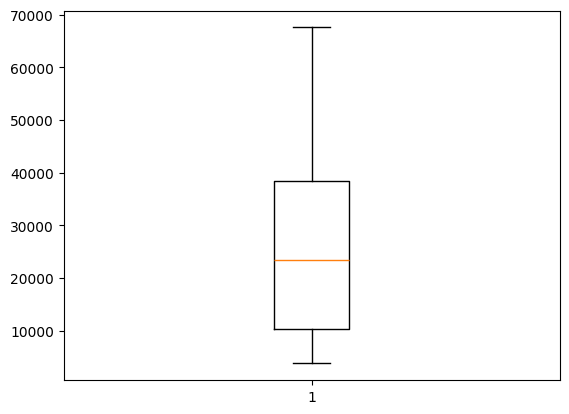
\includegraphics[width=1\textwidth]{bibliography/pictures/BTCboxplot.png}
    \caption{Biểu đồ boxplot về giá đóng phiên của Bitcoin}
    \label{fig:1}
    \end{minipage}
    \hfill
    \begin{minipage}{0.23\textwidth}
    \centering
    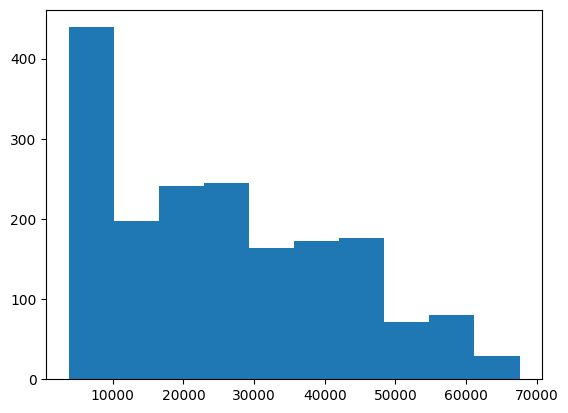
\includegraphics[width=1\textwidth]{bibliography/pictures/BTChistogram.png}
    \caption{Biểu đồ histogram về giá đóng phiên của Bitcoin}
    \label{fig:2}
    \end{minipage}
\end{figure}

\begin{figure}[H]
    \centering
    \begin{minipage}{0.23\textwidth}
    \centering
    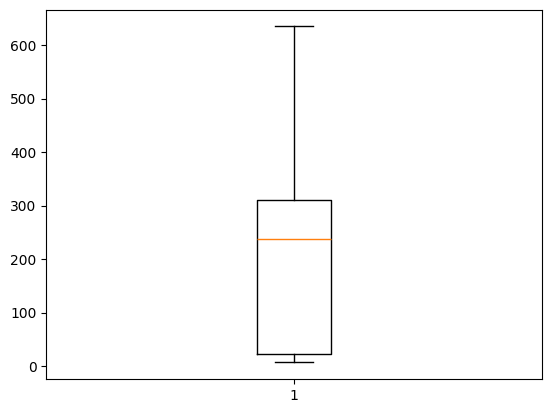
\includegraphics[width=1\textwidth]{bibliography/pictures/BNBboxplot.png}
    \caption{Biểu đồ boxplot về giá đóng phiên của Binance}
    \label{fig:1}
    \end{minipage}
    \hfill
    \begin{minipage}{0.23\textwidth}
    \centering
    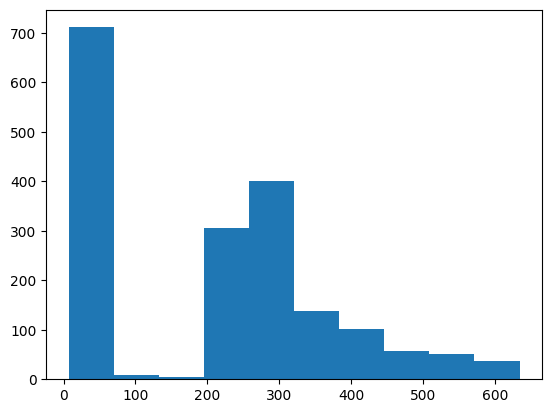
\includegraphics[width=1\textwidth]{bibliography/pictures/BNBhistogram.png}
    \caption{Biểu đồ histogram về giá đóng phiên của Binance}
    \label{fig:2}
    \end{minipage}
\end{figure}

\begin{figure}[H]
    \centering
    \begin{minipage}{0.23\textwidth}
    \centering
    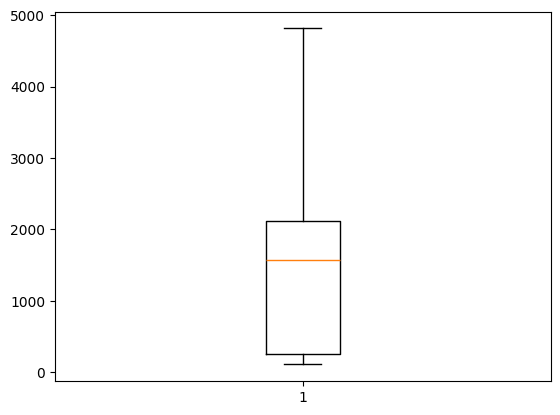
\includegraphics[width=1\textwidth]{bibliography/pictures/ETHboxplot.png}
    \caption{Biểu đồ boxplot về giá đóng phiên của Ethereum}
    \label{fig:1}
    \end{minipage}
    \hfill
    \begin{minipage}{0.23\textwidth}
    \centering
    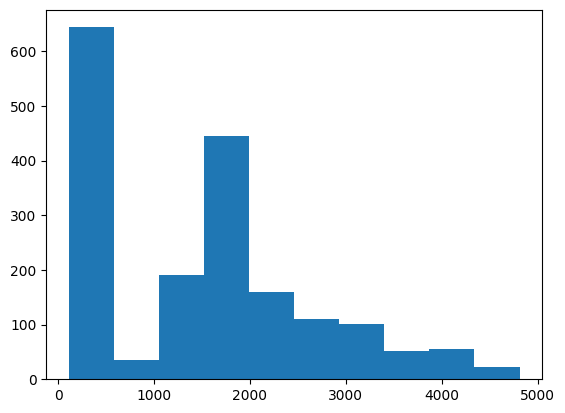
\includegraphics[width=1\textwidth]{bibliography/pictures/ETHhistogram.png}
    \caption{Biểu đồ histogram về giá đóng phiên của Ethereum}
    \label{fig:2}
    \end{minipage}
\end{figure}

Từ hình trên, ta thấy giá của ba loại tiền ảo BNB, BTC và ETH đều có xu hướng lệch phải. Biểu đồ hộp của BNB cho thấy giá trị khá đồng đều và ít biến động, với hộp có kích thước nhỏ và đường râu không kéo dài xa. Ngược lại, biểu đồ hộp của BTC thể hiện sự phân tán và biến động lớn nhất với hộp có kích thước lớn và đường râu kéo dài xa, đặc biệt là phía trên, cho thấy nhiều giá trị ngoại lệ cao. ETH cũng có sự phân tán lớn nhưng ít hơn BTC, với hộp có kích thước tương đối lớn và đường râu kéo dài. Biểu đồ tần suất của cả ba loại tiền ảo cho thấy phần lớn giá trị tập trung ở mức giá thấp hơn, nhưng BTC và ETH có nhiều giá trị ngoại lệ, đặc biệt là BTC. Điều này cho thấy BNB có xu hướng ổn định hơn, trong khi BTC và ETH biến động nhiều hơn, với BTC là loại tiền ảo có biến động lớn nhất.

\section{Methodology}
\subsection{Autoregressive Integrated Moving Average (ARIMA)}
Mô hình ARIMA (Autoregressive Integrated Moving Average) là một phương pháp dự báo thời gian phổ biến trong phân tích dữ liệu và kinh doanh. Mô hình này được Box-Jenkins giới thiệu lần đầu tiên vào năm 1974. Nó được sử dụng để dự đoán giá trị tương lai của dữ liệu chuỗi thời gian, bao gồm các yếu tố thừa kế, xu hướng, chu kỳ và nhiễu.
Mô hình ARIMA là sự kết hợp của 3 thành phần chính: AR (thành phần tự hồi quy); I (tính dừng của chuỗi thời gian); MA (thành phần dự báo trung bình trượt).

Công thức của mô hình ARIMA (p,d,q) có dạng sau:
\[
y_{t} = c + \phi_{1}y_{t-1} + \phi_{2}y_{t-2} + ... + \phi_{p}y_{t-p} + \theta_{1}\epsilon_{t-1} + \theta_{2}\epsilon_{t-2} + ... + \theta_{q}\epsilon_{t-q}
\]
Trong đó:
\begin{itemize}
    \item \(y_{t}\) là giá trị của chuỗi thời gian tại thời điểm t.
    \item c là hằng số.
    \item \(\phi_{1}, \phi_{p}\) là các hệ số Auto Regressive (AR) tương ứng với bậc p.
    \item \(\theta_{1}, \theta_{q}\) là các hệ số Moving Average (MA) tương ứng với bậc q.
    \item \(\epsilon_{t-1}, \epsilon_{t-q}\) là các sai số trước đó được sử dụng để tính toán giá trị hiện tại.
\end{itemize}

Mục đích của mô hình ARIMA là tìm ra các giá trị của các hệ số \(\phi\) và \(\theta\) để dự đoán giá trị của chuỗi thời gian trong tương lai. Quá trình này thường được thực hiện bằng cách sử dụng các phương pháp ước tính thống kê để ước tính các giá trị của các hệ số này từ dữ liệu lịch sử của chuỗi thời gian.

\subsection{Linear Regression}
Hồi quy tuyến tính (Linear regression) là một phương pháp phân tích thống kê dựa trên việc xác định mối quan hệ giữa hai loại biến bao gồm một biến phụ thuộc (kết quả) và các biến độc lập (dự đoán). Mục đích chính của hồi quy tuyến tính là giúp ta dự đoán được giá trị của biến phụ thuộc dựa trên giá trị của các biến độc lập, kiểm tra xem các biến độc lập có ảnh hưởng thế nào đến giá trị của biến phụ thuộc và các biến độc lập nào là yếu tố quan trọng trong việc dự đoán giá trị của biến phụ thuộc. Hồi quy tuyến tính được sử dụng phổ biến và ứng dụng rộng rãi trong nhiều lĩnh vực khác nhau, có thể kể đến như: Y tế, môi trường, giáo dục, kinh tế...
Công thức của mô hình Linear Regression (hồi quy tuyến tính) có dạng như sau:
\begin{itemize}
    \item Đối với hồi quy đơn biến: 
    \[
 Y = \beta_{0}+ \beta_{1}X   
    \] 
    \item Đối với hồi quy đa biến: 
    \[
    Y = \beta_{0} + \beta_{1}X_{1} + \beta_{2}X_{2} + ... + \beta_{p}X_{p}
    \] 
\end{itemize}
Trong đó:
\begin{itemize}
    \item Y là biến đầu ra (target variable) cần được dự đoán.
    \item  \(X_{1}\), \(X_{2}\), ..., \(X_{p}\) là các biến đầu vào (independent variables) được sử dụng để dự đoán Y.
    \item \(\beta_{0}\), \(\beta_{1}\), \(\beta_{2}\), ..., \(\beta_{p}\) là các hệ số (coefficients) tương ứng với mỗi biến đầu vào.
    \item \(\beta_{0}\) là hệ số chặn (intercept) của đường thẳng hoặc siêu phẳng tuyến tính.
    \item \(\beta_{1}\), \(\beta_{2}\), ..., \(\beta_{p}\) là hệ số hồi quy (regression coefficients) cho biến đầu vào tương ứng.
\end{itemize}

\subsection{Holt-Winters}
Mô hình Holt-Winters là một mô hình dự báo chuỗi thời gian bằng cách sử dụng exponential smoothing. Mô hình này chú trọng đến ba thành phần của một chuỗi thời gian: mức độ (level), xu hướng (trend) và tính thời vụ (seasonality), đồng thời sử dụng chúng để đưa ra các dự báo trong tương lai.
Mô hình Holt-Winters được chia thành hai loại: Additive Holt-Winters (AH-W) và Multiplicative Holt-Winters (MH-W)

\[
l_{t} = (1 - \alpha)l_{t - 1} + \alpha x_{t}
\]
\[
b_{t} = (1 - \beta)b_{t - 1} + \beta (l_{t} - l_{t - 1})
\]
\[
c_{t} = (1 - \gamma)c_{t - L} + \gamma (x_{t} - l_{t - 1} - b_{t - 1})
\]
\[
y_{t} = (l_{t} + b_{t})c_{t}
\]
Trong đó:
\begin{itemize}
    \item \(\alpha\) là hệ số làm mịn theo mức độ (level).
    \item \(\beta\) là hệ số làm mịn theo xu hướng (trend).
    \item \(\gamma\) là hệ số làm mịn theo mùa (season).
\end{itemize}
Với \(0 \leq \gamma \leq 1-\alpha\)

\subsection{Gradient Boosting regression}
Gradient Boosting là một thuật toán máy học được sử dụng để giải quyết các bài toán hồi quy, trong đó các mô hình yếu được xây dựng tuần tự, mỗi mô hình cố gắng sửa lỗi của mô hình trước đó. 
Giả sử chúng ta có $M$ mô hình, dự đoán của mô hình Gradient Boosting có thể được biểu diễn như sau:
\[
F_M(x) = F_{M-1}(x) + \alpha \cdot h_M(x)
\]
Trong đó:
\begin{itemize}
    \item $F_M(x)$ là dự đoán cuối cùng sau $M$ lần lặp.
    \item $F_{M-1}(x)$ là dự đoán từ lần lặp thứ $M-1$.
    \item $h_M(x)$ là mô hình mới (thường là một cây quyết định) được huấn luyện trên các residuals.
    \item $\alpha$ là learning rate.
\end{itemize}

\subsection{Bagging Model-RandomForest}
Random Forest:
Random Forests là thuật toán học có giám sát (supervised learning). Nó có thể được sử dụng cho cả phân lớp và hồi quy. Nó cũng là thuật toán linh hoạt và dễ sử dụng nhất. Một khu rừng bao gồm cây cối. Người ta nói rằng càng có nhiều cây thì rừng càng mạnh. Random forests tạo ra cây quyết định trên các mẫu dữ liệu được chọn ngẫu nhiên, được dự đoán từ mỗi cây và chọn giải pháp tốt nhất bằng cách bỏ phiếu. Nó cũng cung cấp một chỉ báo khá tốt về tầm quan trọng của tính năng. Random forests có nhiều ứng dụng, chẳng hạn như công cụ đề xuất, phân loại hình ảnh và lựa chọn tính năng. Nó có thể được sử dụng để phân loại các ứng viên cho vay trung thành, xác định hoạt động gian lận và dự đoán các bệnh. Nó nằm ở cơ sở của thuật toán Boruta, chọn các tính năng quan trọng trong tập dữ liệu.
Random Forest hoạt động theo 4 bước:
\begin{itemize}
    \item Chọn các mẫu ngẫu nhiên từ tập dữ liệu đã cho.
    \item Thiết lập cây quyết định cho từng mẫu và nhận kết quả dự đoán từ mỗi cây quyết định.
    \item Bỏ phiếu cho mỗi kết quả dự đoán.
    \item Chọn kết quả được dự đoán nhiều nhất là dự đoán cuối cùng.
\end{itemize}

\begin{figure} [H]
    \centering
    \begin{minipage}{0.3\textwidth}
    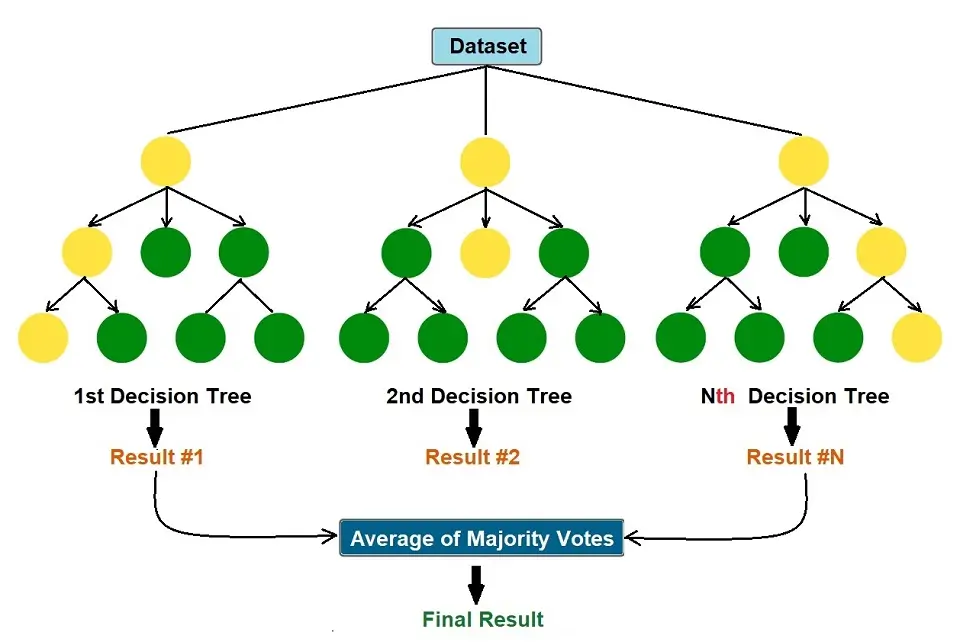
\includegraphics[width=1\textwidth]{bibliography/pictures/RandomForest.jpg}
    \caption{Mô hình của Random Forest}
    \end{minipage}  
\end{figure}

\subsection{Recurrent Neural Networks (RNN)} 
Mô hình RNN (Recurrent Neural Network) giữ một trạng thái ẩn (hidden state) và sử dụng nó để lưu trữ thông tin từ các bước thời gian trước đó. Điều này cho phép RNN hiểu và xử lý các dữ liệu dạng chuỗi, chẳng hạn như văn bản, âm thanh hoặc dữ liệu thời gian.

\begin{figure}[H]
    \centering
    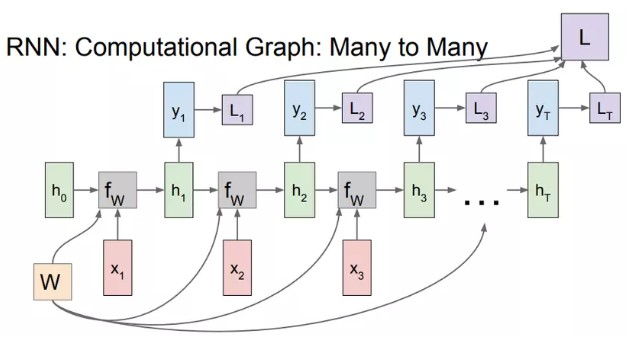
\includegraphics[width=0.4\textwidth]{bibliography/pictures/RNN.jpg}
    \caption{Mô hình Many to Many}
\end{figure}

\begin{itemize}  
    \item \textbf{Mô hình Many to Many của RNN:}
    \begin{itemize}
        \item Mạng Neural Network thông thường bao gồm các lớp: lớp đầu vào (input layer) \( x \), lớp ẩn (hidden layer) \( h \), và lớp đầu ra (output layer) \( y \). Tất cả các lớp này được kết nối đầy đủ với nhau.
        \item Trong RNN, đầu vào tại mỗi thời điểm \( x_t \) sẽ được kết hợp với lớp ẩn từ bước thời gian trước đó \( h_{t-1} \) thông qua hàm \( f_W \) để tính toán ra lớp ẩn hiện tại \( h_t \). Đầu ra tại mỗi thời điểm \( y_t \) sẽ được tính từ lớp ẩn hiện tại \( h_t \), W là tập các trọng số và nó được xuất hiện ở tất cả các cụm, các \( L_1, L_2, \ldots, L_T \) là các hàm mất mát.
        \item Kết quả của các quá trình tính toán trước đã được "nhớ" bằng cách kết hợp thêm \( h_{t-1} \) để tính toán \( h_t \). Điều này giúp tăng độ chính xác cho những dự đoán ở hiện tại.
        \item Hàm \( f_W \) kết hợp \( h_{t-1} \) và \( x_t \) để tính \( h_t \):
        \[
        h_t = f_W(h_{t-1}, x_t)
        \]
        \item Hàm \( f_W \) được định nghĩa cụ thể là hàm \( \tanh \), công thức trên sẽ trở thành:
        \[
        h_t = \tanh(W_{hh}h_{t-1} + W_{xh}x_t)
        \]
        \item Đầu ra \( y_t \) được tính từ \( h_t \):
        \[
        y_t = W_{hy}h_t
        \]
        \item RNN sử dụng 3 ma trận trọng số là \( W_{hh} \) kết hợp với "bộ nhớ trước" \( h_{t-1} \) và \( W_{xh} \) kết hợp với đầu vào hiện tại \( x_t \) để tính toán "bộ nhớ của bước hiện tại" \( h_t \) từ đó kết hợp với \( W_{hy} \) để tính toán đầu ra \( y_t \).
    \end{itemize}
            
    \item \textbf{Các Dạng Mô Hình RNN Khác:}
    \begin{itemize}
        \item Ngoài mô hình Many to Many, RNN còn có các dạng khác như One to One, One to Many, Many to One.
    \end{itemize}
\end{itemize}

\subsection{LSTM}

LSTM (Bộ nhớ dài hạn) là một loại mạng nơ-ron hồi quy (RNN) được giới thiệu bởi Hochreiter và Schmidhuber vào năm 1997. Nó được thiết kế để khắc phục những hạn chế của RNN truyền thống trong việc nắm bắt và ghi nhớ các phụ thuộc dài hạn trong dữ liệu tuần tự.

Ý tưởng chính của LSTM xoay quanh khái niệm về trạng thái tế bào hoặc bộ nhớ. Trạng thái tế bào hoạt động như một băng tải, cho phép thông tin chảy qua mạng lưới trong khi vẫn giữ được thông tin quan trọng qua các chuỗi dài. Tế bào LSTM bao gồm một số thành phần: một cổng đầu vào, một cổng quên, một cổng đầu ra, và một cơ chế cập nhật tế bào.
\begin{figure}[h]
    \centering
    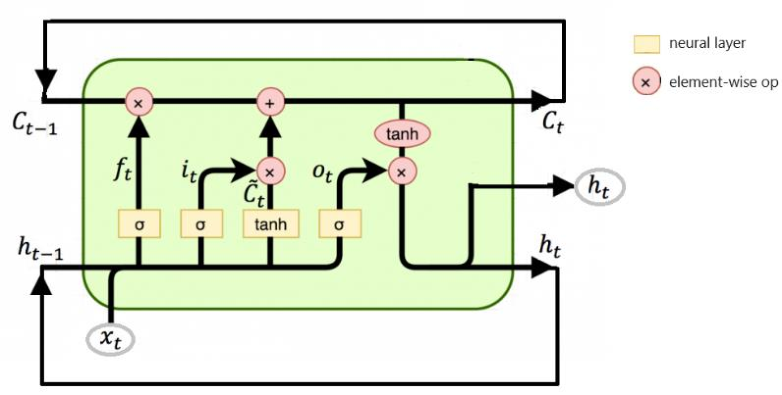
\includegraphics[width=0.4\textwidth]{bibliography/pictures/lstm.png}
  \caption{Cấu trúc của LSTM.}
\end{figure}
Các công thức để tính các thành phần khác nhau của tế bào LSTM như sau: 


\begin{align*}
\text{Cổng đầu vào:} \quad & i_t = \sigma(W_i * [h_{t-1}, x_t] + b_i) \\
\text{Cổng quên:} \quad & f_t = \sigma(W_f * [h_{t-1}, x_t] + b_f) \\
\text{Cập nhật tế bào:} \quad & \tilde{C}_t = \tanh(W_c * [h_{t-1}, x_t] + b_c) \\
\text{Trạng thái tế bào:} \quad & C_t = f_t * C_{t-1} + i_t * \tilde{C}_t \\
\text{Cổng đầu ra:} \quad & o_t = \sigma(W_o * [h_{t-1}, x_t] + b_o) \\
\text{Trạng thái ẩn:} \quad & h_t = o_t * \tanh(C_t)
\end{align*}

Trong các công thức này, $W_i$, $W_f$, $W_c$, $W_o$ đại diện cho ma trận trọng số, $b_i$, $b_f$, $b_c$, $b_o$ đại diện cho vector độ lệch, $h_{t-1}$ đại diện cho trạng thái ẩn trước đó, $x_t$ đại diện cho đầu vào tại thời điểm $t$, và $*$ biểu thị phép nhân ma trận.

\subsection{LIGHTGBM}
LightGBM là một thư viện học máy gradient boosting mạnh mẽ và nhanh chóng được phát triển bởi Microsoft. LightGBM sử dụng các thuật toán dựa trên cây quyết định để cải thiện hiệu suất và tốc độ của các mô hình dự đoán.

Ý tưởng chính của LightGBM là tạo ra các cây quyết định dựa trên kỹ thuật gradient boosting. Thay vì xây dựng các cây lớn và phức tạp, LightGBM xây dựng các cây nhỏ và tối ưu chúng để giảm thiểu sai số dự đoán. Một số ưu điểm của LightGBM bao gồm: tốc độ huấn luyện nhanh, khả năng mở rộng lớn, và hỗ trợ nhiều tính năng tiên tiến như xử lý dữ liệu thiếu và hỗ trợ cho các mô hình tuần tự.

\begin{figure}[H]
    \centering
    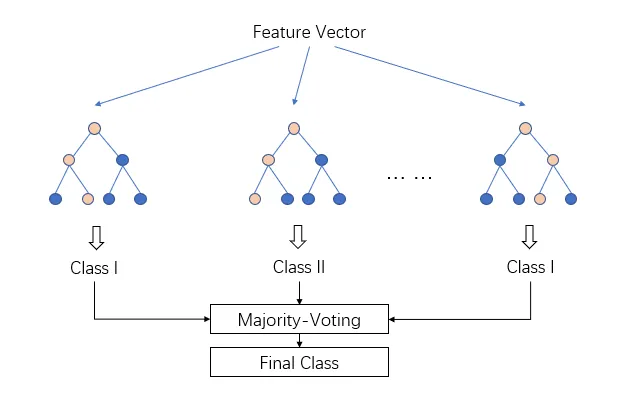
\includegraphics[width=0.4\textwidth]{bibliography/pictures/lightgbm.png}
    \caption{Cấu trúc của LightGBM.}
\end{figure}

Các công thức để tính các thành phần khác nhau của LightGBM như sau: 
\[
Hàm mất mát: L(y, \hat{y}) = \sum_{i=1}^{n} \text{loss}(y_i, \hat{y}_i)
\]
\[
Gradient: g_i = \frac{\partial L(y_i, \hat{y}_i)}{\partial \hat{y}_i}
\]
\[
Hessian: h_i = \frac{\partial^2 L(y_i, \hat{y}_i)}{\partial \hat{y}_i^2}
\]
Giá trị phân chia tốt nhất:
\[
\text{Split\_value} = \arg\min_{s} \left[ \frac{(\sum_{i \in I_L} g_i)^2}{\sum_{i \in I_L} h_i + \lambda} + \frac{(\sum_{i \in I_R} g_i)^2}{\sum_{i \in I_R} h_i + \lambda} \right]
\]

Trong các công thức này, $y$ đại diện cho nhãn thực tế, $\hat{y}$ đại diện cho dự đoán của mô hình, $g_i$ là gradient, $h_i$ là Hessian, $I_L$ và $I_R$ lần lượt là các chỉ số của các mẫu trong nút trái và phải, và $\lambda$ là tham số điều chỉnh.
\subsection{PatchTST}
Các phương pháp truyền thống gặp khó khăn trong việc dự báo dài hạn trong dữ liệu chuỗi thời gian. Một trong những giải pháp cho vấn đề này là mô hình Patch-based Time Series Transformer (PatchTST). Mô hình này chia dữ liệu thành các phân đoạn nhỏ hơn (patches) và sử dụng kiến trúc Transformer để nắm bắt các phụ thuộc tầm xa trong các phân đoạn đó.

\begin{figure}[H]
    \centering
    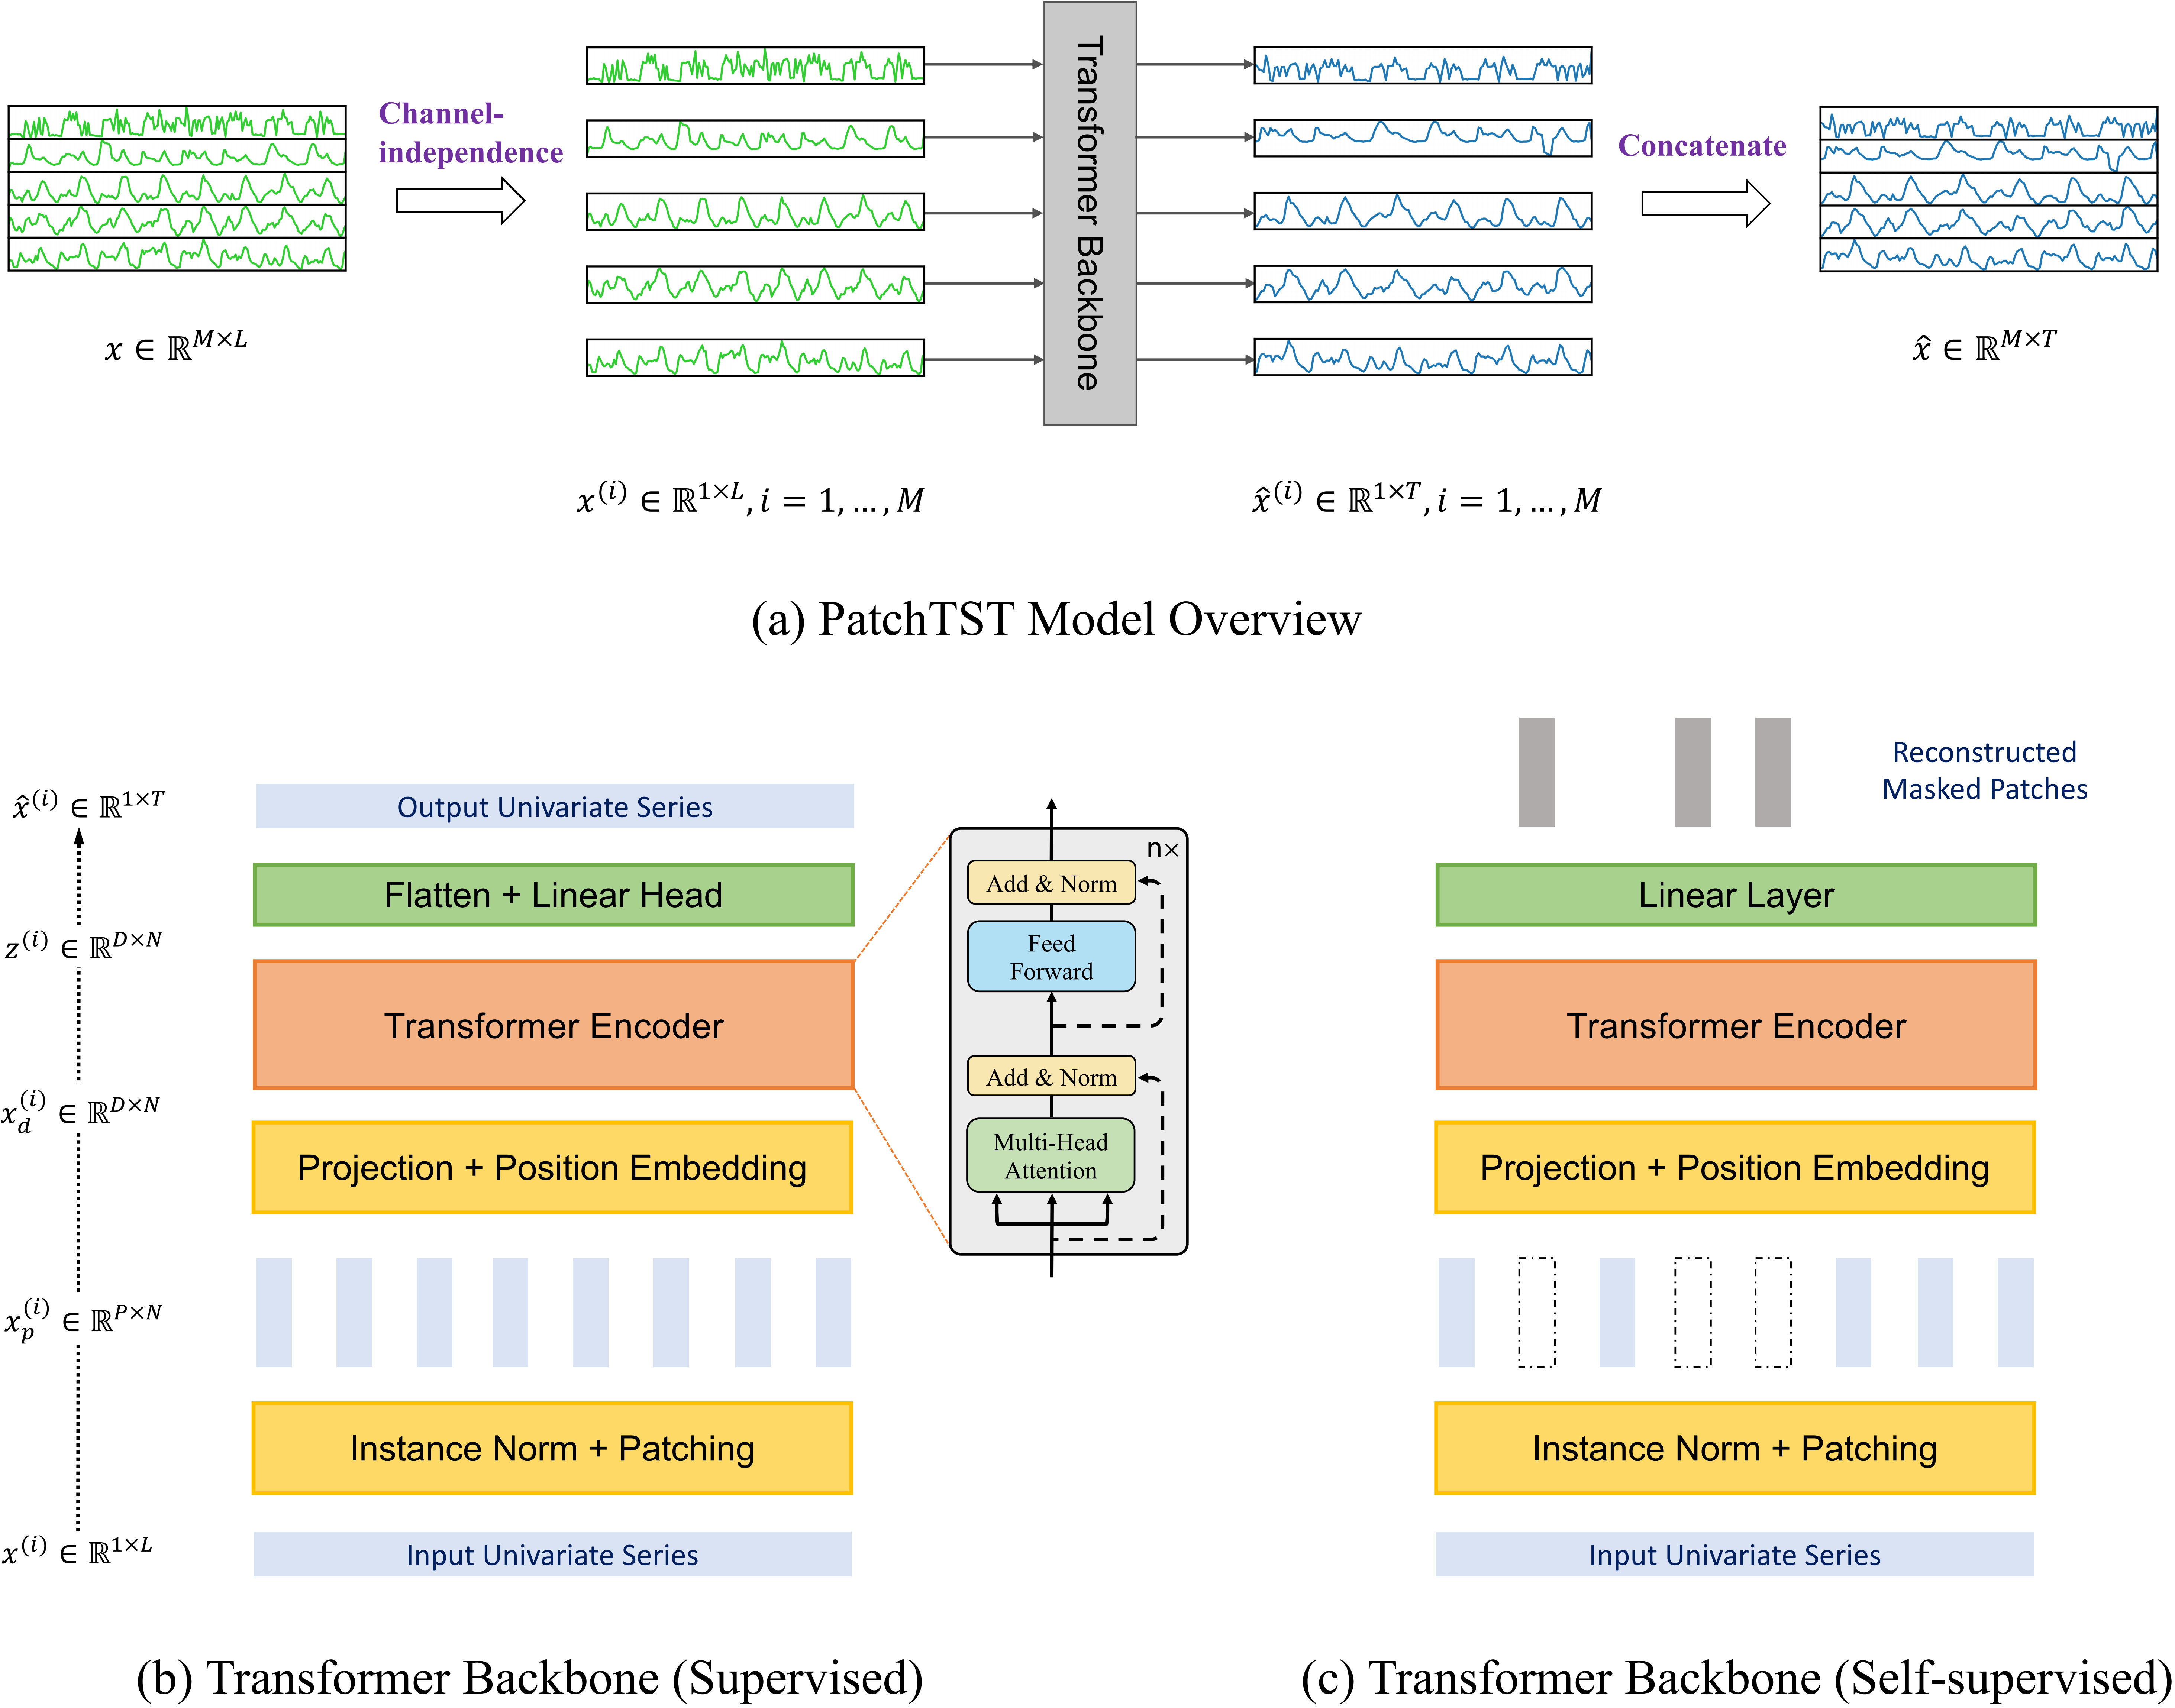
\includegraphics[width=0.3\textwidth]{bibliography/pictures/modelPatchTST.png}
    \caption{Mô hình PatchTST.}
\end{figure}
Hình (a): Dữ liệu chuỗi thời gian đa biến được chia thành các kênh khác nhau. Chúng cùng chia sẻ một backbone Transformer, nhưng các quá trình hướng tới (forward processes) là độc lập.
Hình (b): Mỗi kênh đơn biến được truyền qua toán tử chuẩn hóa theo từng cá thể (instance normalization) và được chia thành các bản vá. Các bản vá này được sử dụng làm token đầu vào của Transformer.
Hình (c): Học biểu diễn tự giám sát có mặt nạ với PatchTST, trong đó các bản vá được chọn ngẫu nhiên và đặt thành bằng không. Mô hình sẽ tái tạo các bản vá bị che khuất.

\subsection{Gated Recurrent Unit (GRU)}
GRU là một mô hình RNN mạng nơ ron và là một biến thể đơn giản của LSTM nhưng thường đạt chất lượng huấn luyện model tương đương và tính toán nhanh đáng kể. GRU có ứng dụng lớn trong xử lí ngôn ngữ tự nhiên, nhận dạng giọng nói, nhận dạng hình ảnh và dự đoán chuỗi thời gian. Với cấu trúc đơn giản hơn LSTM giúp việc đào tạo trở nên dễ dàng với chuỗi liệu dài hơn. 
GRU hoạt động theo các bước sau:
\begin{itemize}
    \item Tính toán trạng thái ẩn dự đoán: Sử dụng thông tin đầu vào hiện tại và trạng thái ẩn trước đó để tính toán một trạng thái ẩn dự đoán.
    \item Cập nhật cổng cập nhật: Sử dụng thông tin đầu vào hiện tại và trạng thái ẩn trước đó để tính toán giá trị của cổng cập nhật.
    \item Cập nhật cổng đặt lại: Sử dụng thông tin đầu vào hiện tại và trạng thái ẩn trước đó để tính toán giá trị của cổng đặt lại.
    \item Tính toán trạng thái ẩn: Sử dụng trạng thái ẩn dự đoán, cổng cập nhật, cổng đặt lại và trạng thái ẩn trước đó để tính toán trạng thái ẩn.
\end{itemize}
\begin{figure}[H]
    \centering
    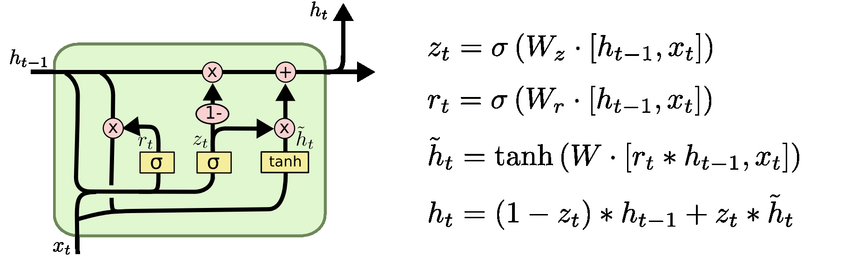
\includegraphics[width=0.4\textwidth]{bibliography/pictures/GRU.png}
    \caption{Mô hình GRU.}
\end{figure}
\section{Experiment}
\subsection{Evaluation Metrics} 
\subsubsection{Mean Squared Error (MSE)} là trung bình của bình phương các sai số, tức là sự khác biệt giữa các ước lượng và những gì được đánh giá. Giá trị MSE càng thấp, tức là sự khác biệt giữa giá trị dự báo và giá trị thực tế càng nhỏ thì mô hình dự báo càng tốt. Công thức tính MSE như sau:
\[
\text{MSE} = \frac{1}{n} \sum_{i=1}^{n} (y_i - \hat{y}_i)^2
\]
\subsubsection{Root Mean Square Error (RMSE)} đo lường sai số trung bình của mô hình so với dữ liệu thực tế. RMSE được tính bằng căn bậc hai của trung bình bình phương của sai số giữa giá trị dự đoán và giá trị thực tế. Giá trị RMSE càng nhỏ thì mô hình càng tốt. Công thức tính RMSE như sau:
\[
\text{RMSE} = \sqrt{\frac{1}{n} \sum_{i=1}^{n} (y_i - \hat{y}_i)^2}
\]
\subsubsection{Mean Absolute Percentage Error (MAPE)} đo lường tỉ lệ phần trăm trung bình của sai số giữa giá trị dự đoán và giá trị thực tế. MAPE được tính bằng trung bình giá trị tuyệt đối của sai số chia cho giá trị thực tế, nhân với 100. Giá trị MAPE càng nhỏ thì mô hình càng tốt. Công thức tính MAPE như sau:
\[
\text{MAPE} = \frac{1}{n} \sum_{i=1}^{n} \left| \frac{y_i - \hat{y}_i}{y_i} \right| \times 100
\]

\subsection{Model Setting}

\subsubsection{Arima}



\subsubsection{GRU}
\begin{figure}[H]
    \centering
    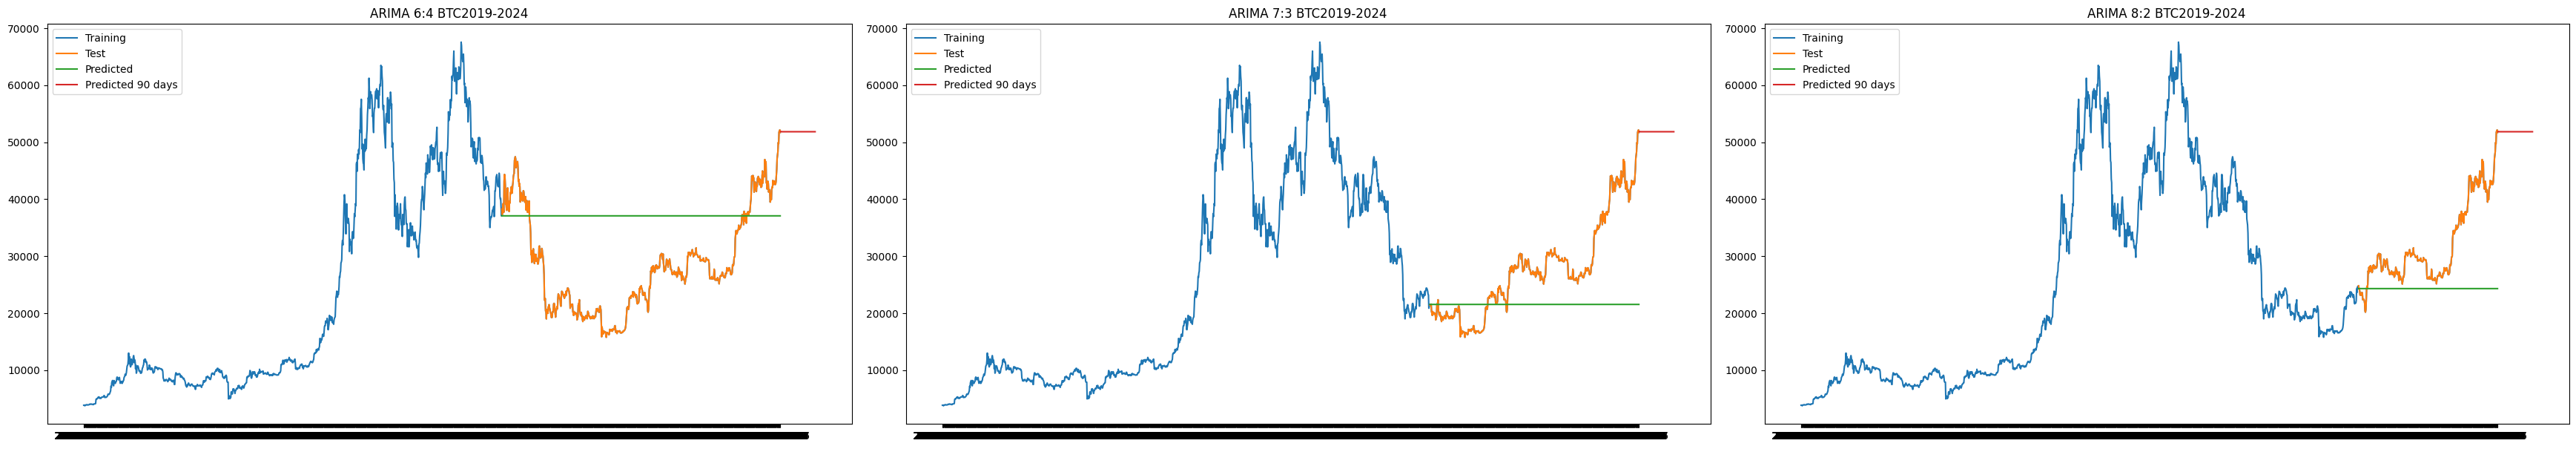
\includegraphics[width=0.5\textwidth]{bibliography/Figure/ARIMA_BTC_90.png}
    \caption{Kết quả dự đoán giá Bitcoin của ARIMA}
\end{figure}
\begin{figure}[H]
    \centering
    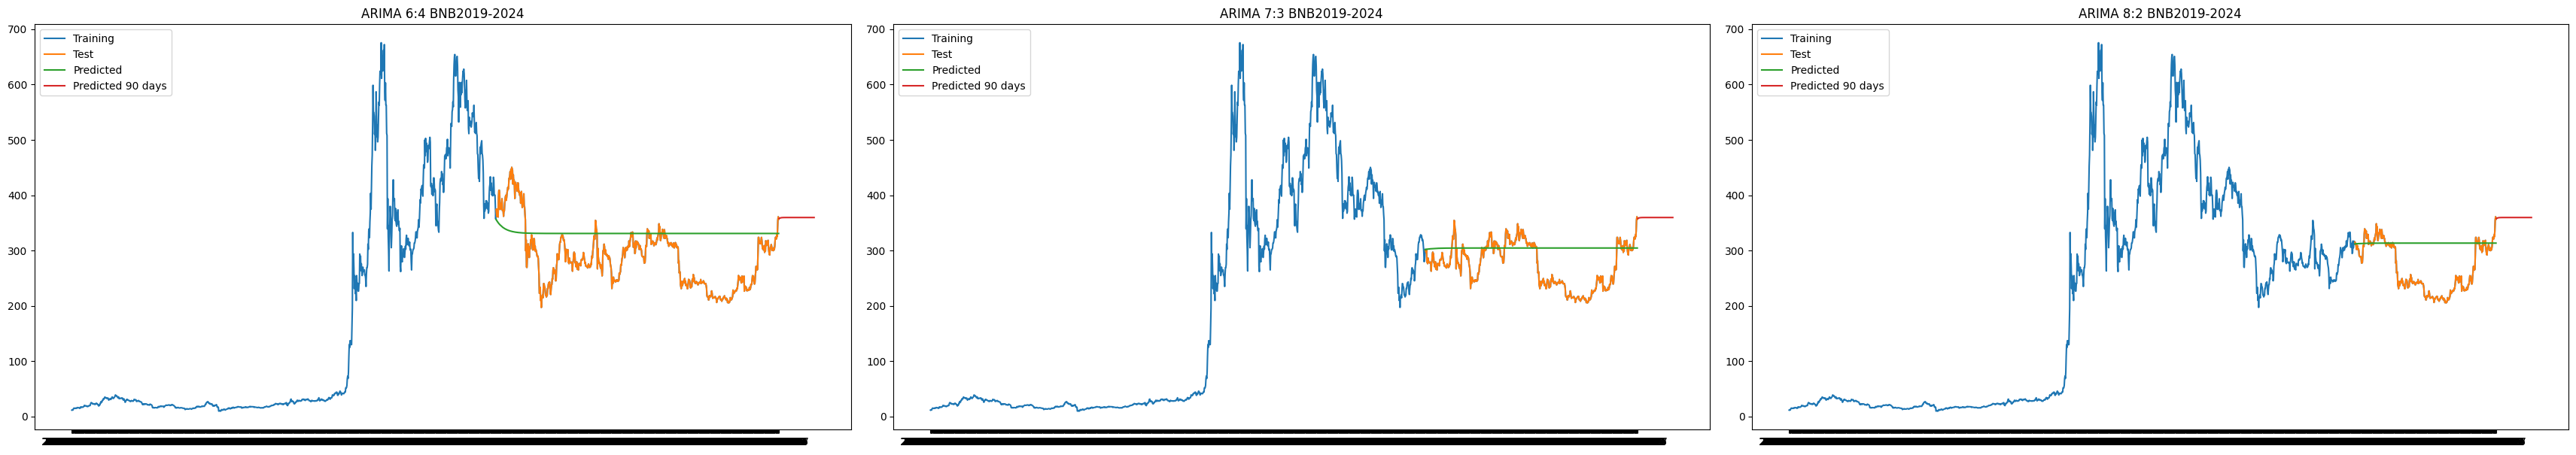
\includegraphics[width=0.5\textwidth]{bibliography/Figure/ARIMA_BNB_90.png}
    \caption{Kết quả dự đoán giá Binance của ARIMA}
\end{figure}
\begin{figure}[H]
    \centering
    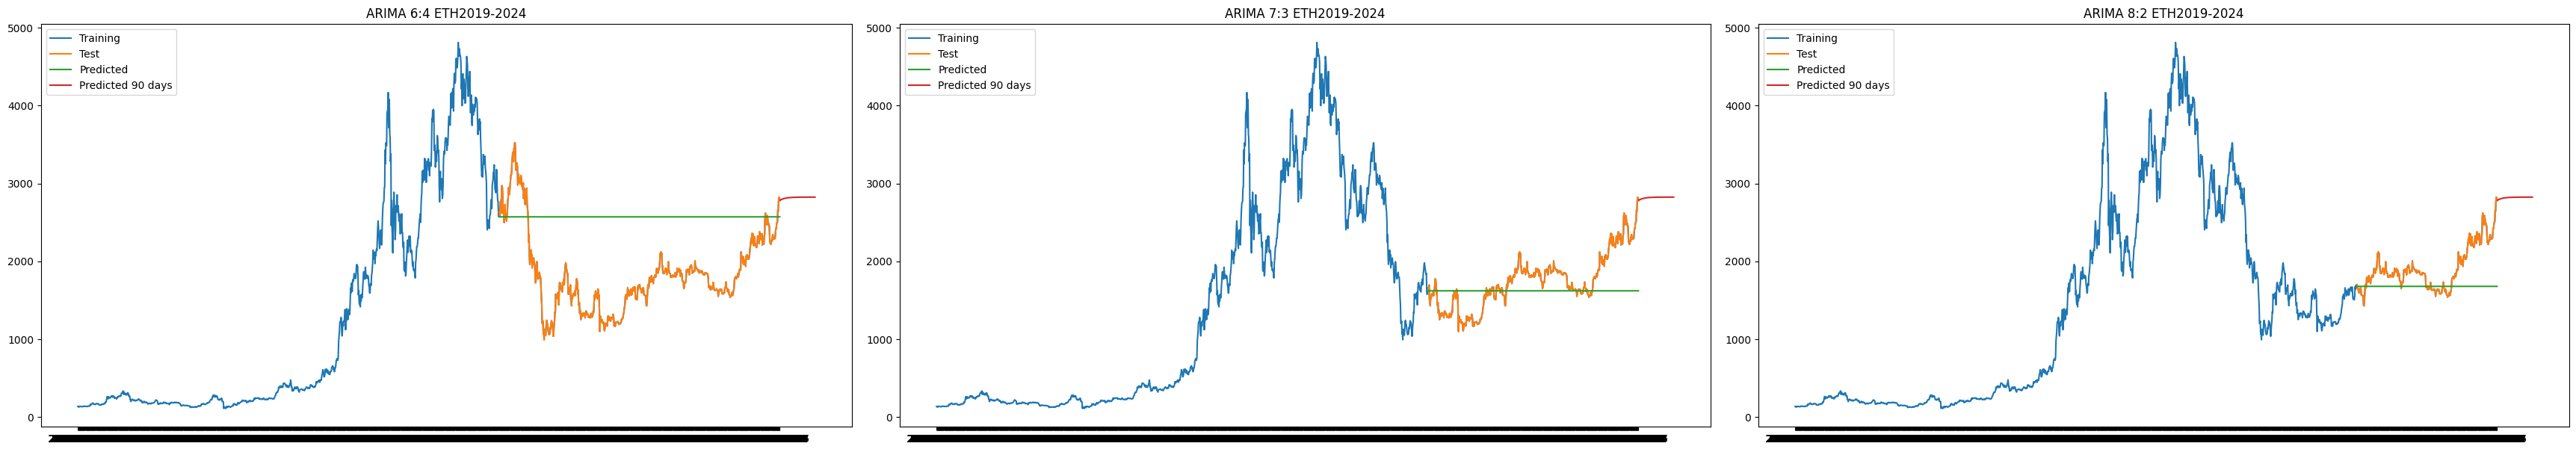
\includegraphics[width=0.5\textwidth]{bibliography/Figure/ARIMA_ETH_90.png}
    \caption{Kết quả dự đoán giá Ethereum của ARIMA}
\end{figure}




\subsubsection{Gradient Boosting}

\begin{figure}[H]
    \centering
    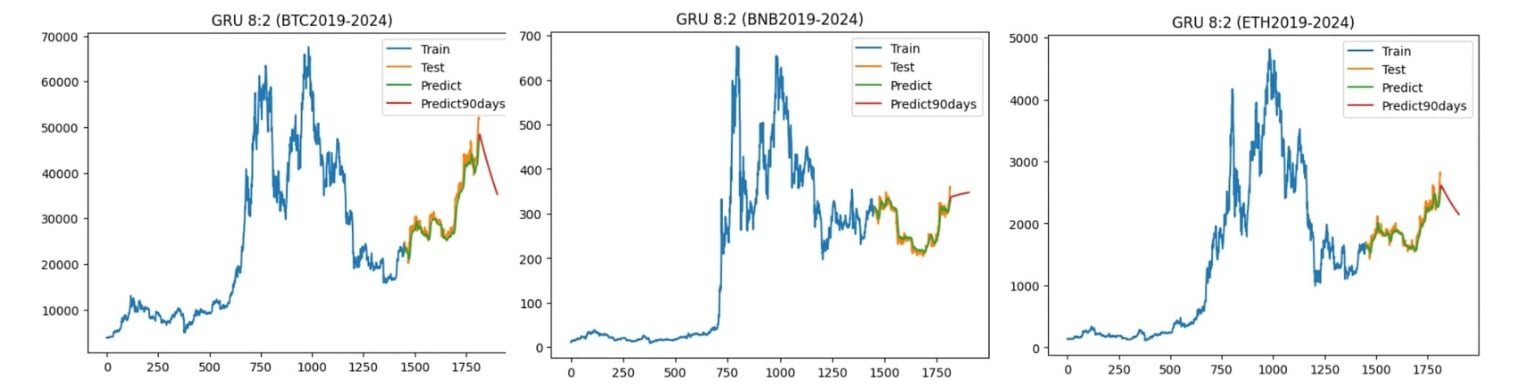
\includegraphics[width=0.5\textwidth]{bibliography/pictures/GRU_82.jpg}
    \caption{Kết quả dự đoán giá của GRU với tỉ lệ 8:2.}
\end{figure}
\begin{figure}[H]
    \centering
    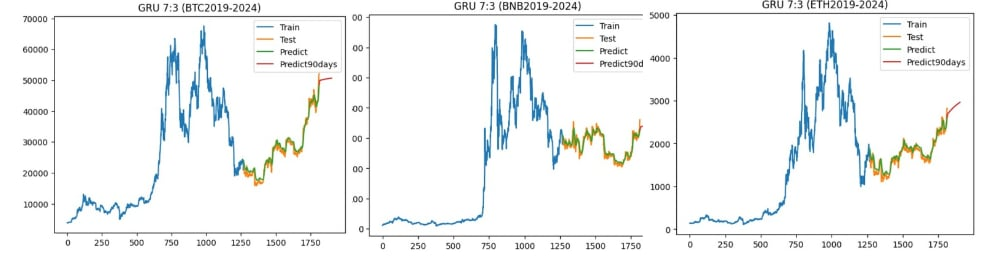
\includegraphics[width=0.5\textwidth]{bibliography/pictures/GRU_73.jpg}
    \caption{Kết quả dự đoán giá của GRU với tỉ lệ 7:3.}
\end{figure}
\begin{figure}[H]
    \centering
    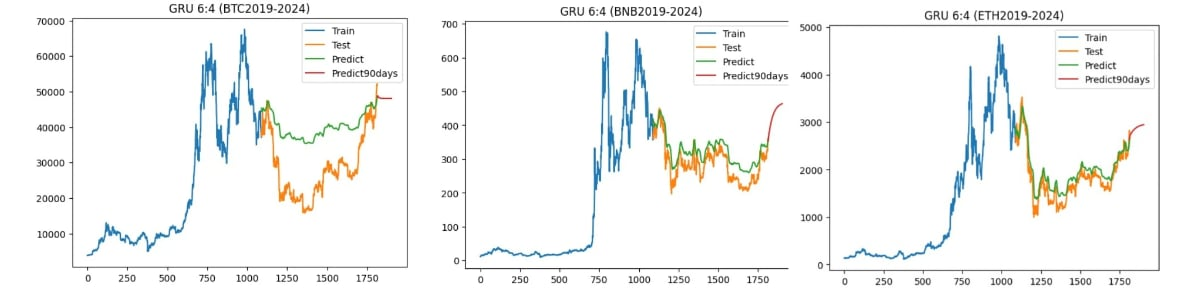
\includegraphics[width=0.5\textwidth]{bibliography/pictures/GRU_64.jpg}
    \caption{Kết quả dự đoán giá của GRU với tỉ lệ 6:4.}
\end{figure}

\subsubsection{LSTM}

\begin{figure}[H]
    \centering
    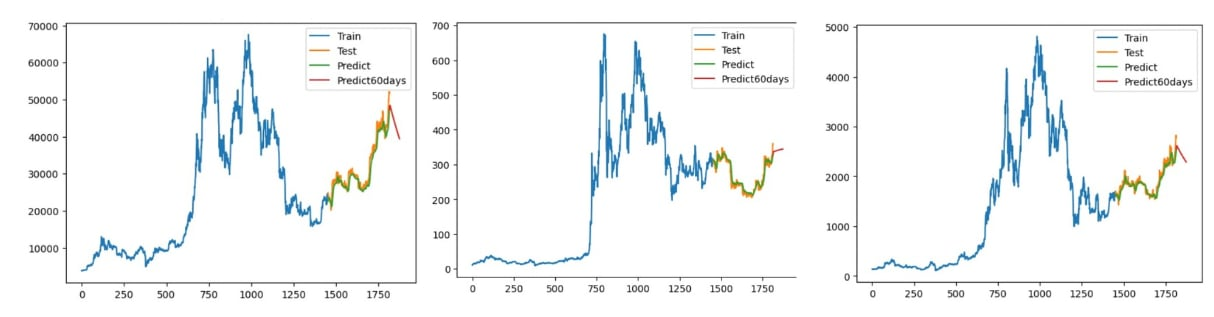
\includegraphics[width=0.5\textwidth]{bibliography/pictures/GB_82.jpg}
    \caption{Kết quả dự đoán giá của GB với tỉ lệ 8:2.}
\end{figure}
\begin{figure}[H]
    \centering
    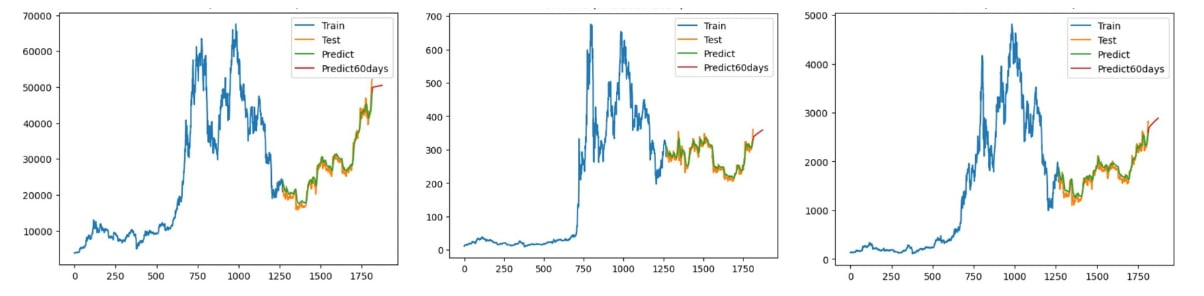
\includegraphics[width=0.5\textwidth]{bibliography/pictures/GB_73.jpg}
    \caption{Kết quả dự đoán giá của GB với tỉ lệ 7:3.}
\end{figure}
\begin{figure}[H]
    \centering
    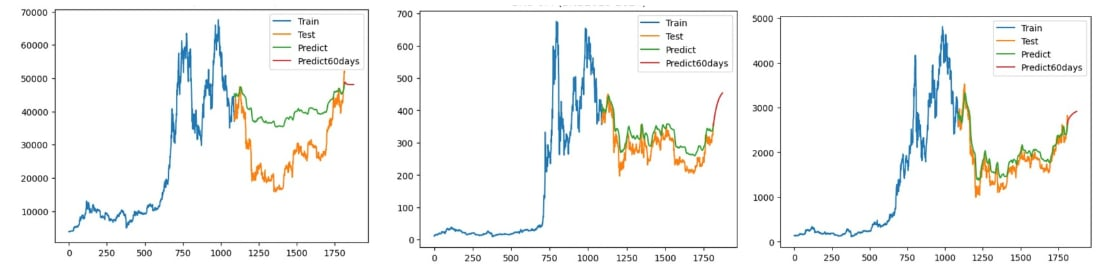
\includegraphics[width=0.5\textwidth]{bibliography/pictures/GB_64.jpg}
    \caption{Kết quả dự đoán giá của GB với tỉ lệ 6:4.}
\end{figure}



\subsubsection{LightGBM}

\begin{figure}[H]
    \centering
    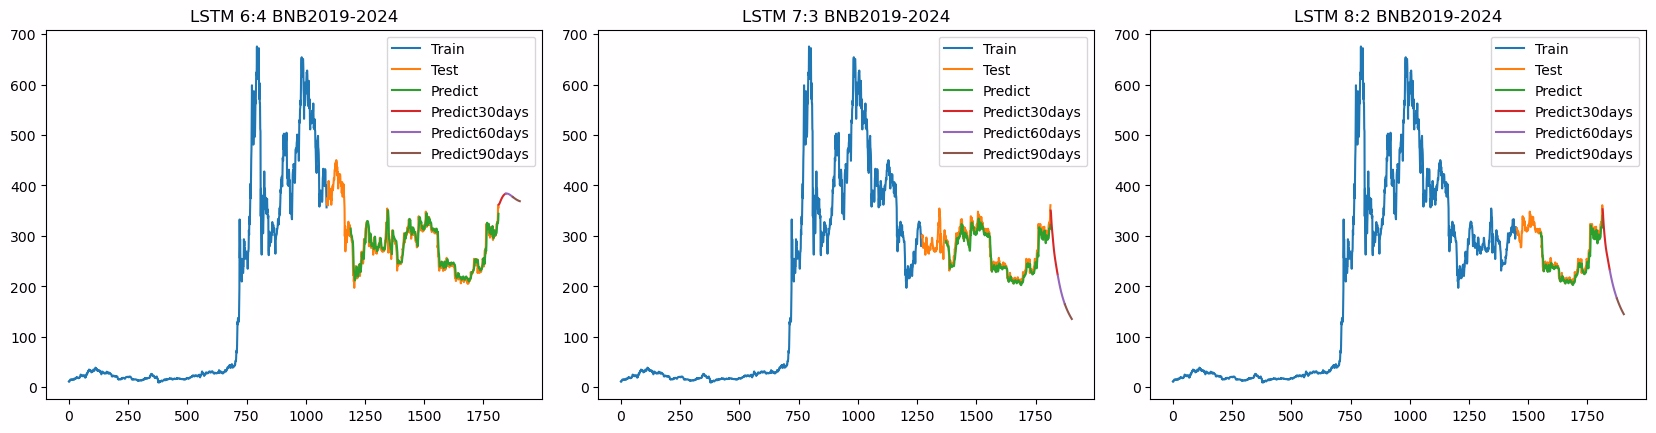
\includegraphics[width=0.5\textwidth]{bibliography/pictures/LSTM BNB.jpg}
    \caption{Kết quả dự đoán giá Binance của LSTM.}
\end{figure}

\begin{figure}[H]
    \centering
    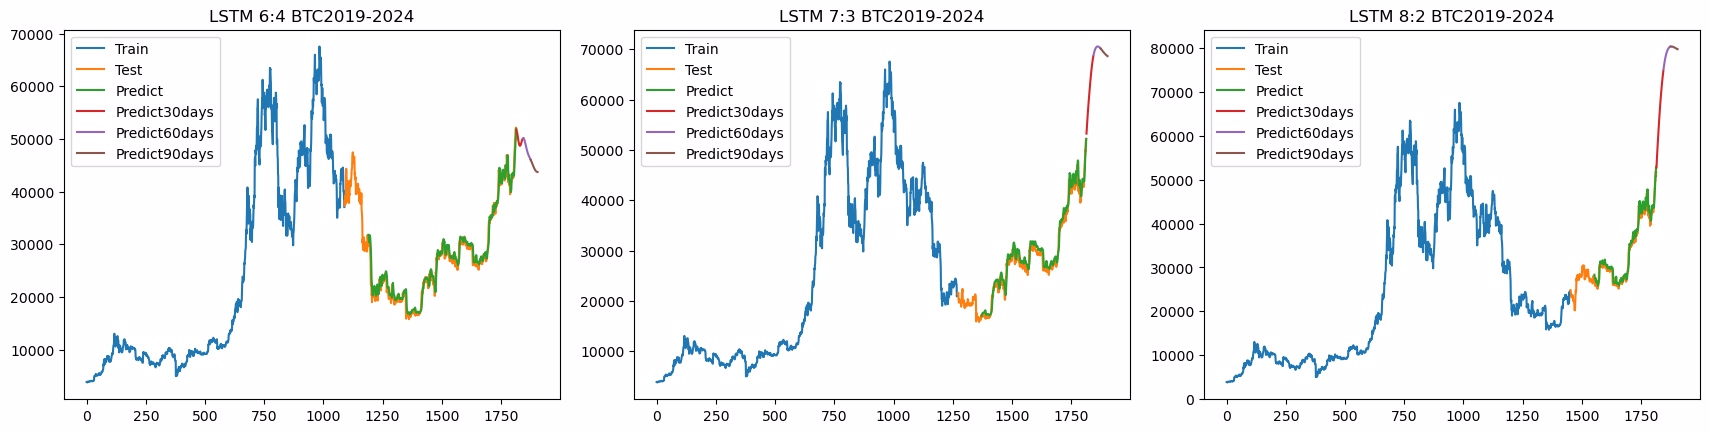
\includegraphics[width=0.5\textwidth]{bibliography/pictures/LSTM BTC.jpg}
    \caption{Kết quả dự đoán giá Bitcoin của LSTM.}
\end{figure}

\begin{figure}[H]
    \centering
    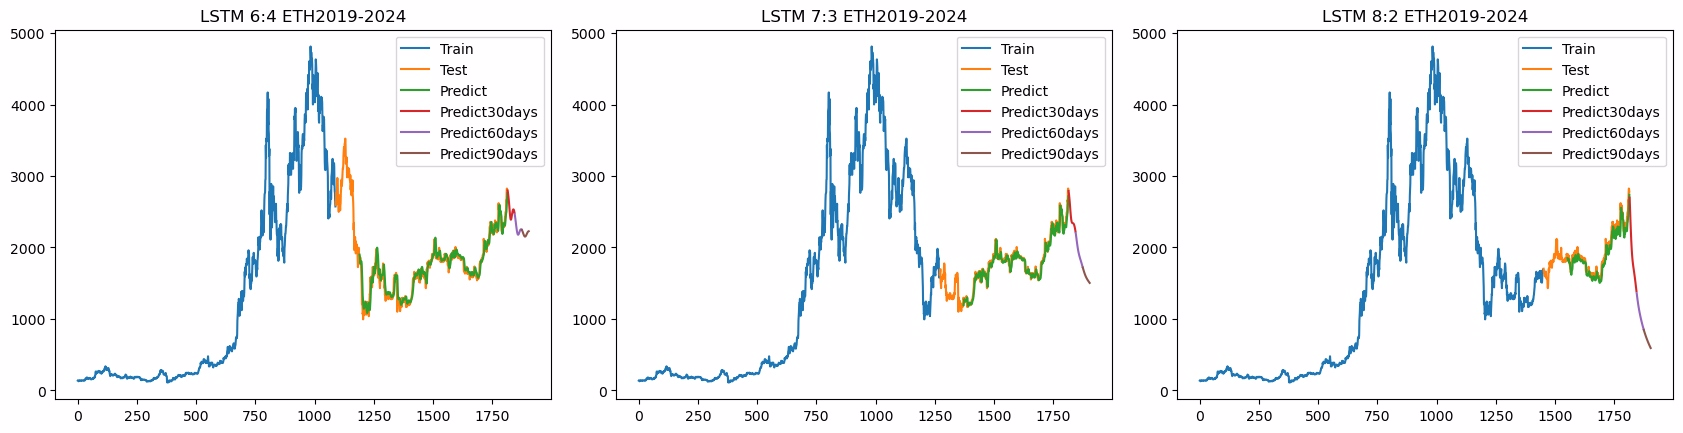
\includegraphics[width=0.5\textwidth]{bibliography/pictures/LSTM ETH.jpg}
    \caption{Kết quả dự đoán giá Ethereum của LSTM.}
\end{figure}



\subsubsection{RNN}

\begin{figure}[H]
    \centering
    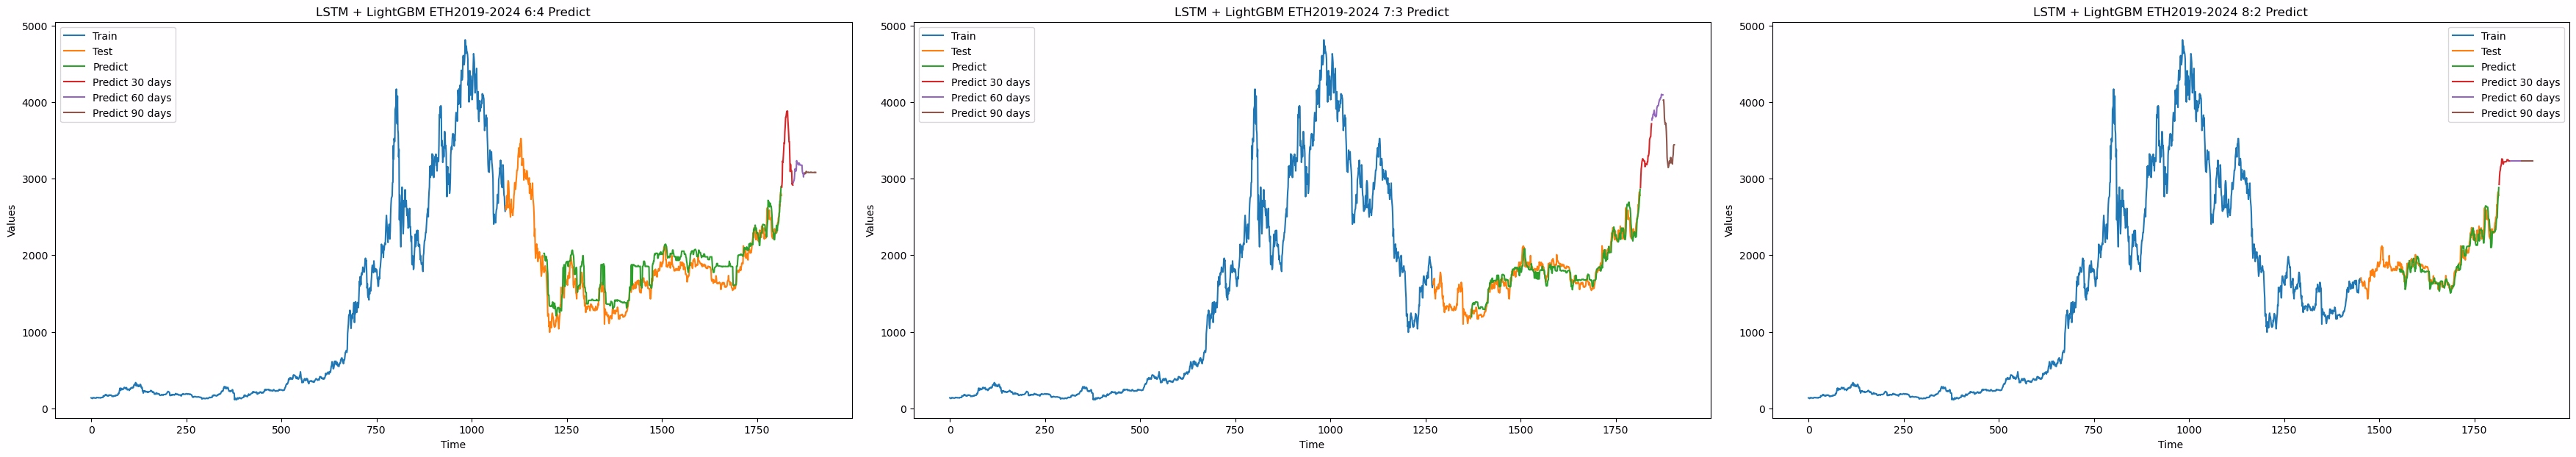
\includegraphics[width=0.5\textwidth]{bibliography/pictures/ETH LightGBM.jpg}
    \caption{Kết quả dự đoán giá Ethereum của LightGBM.}
\end{figure}
\begin{figure}[H]
    \centering
    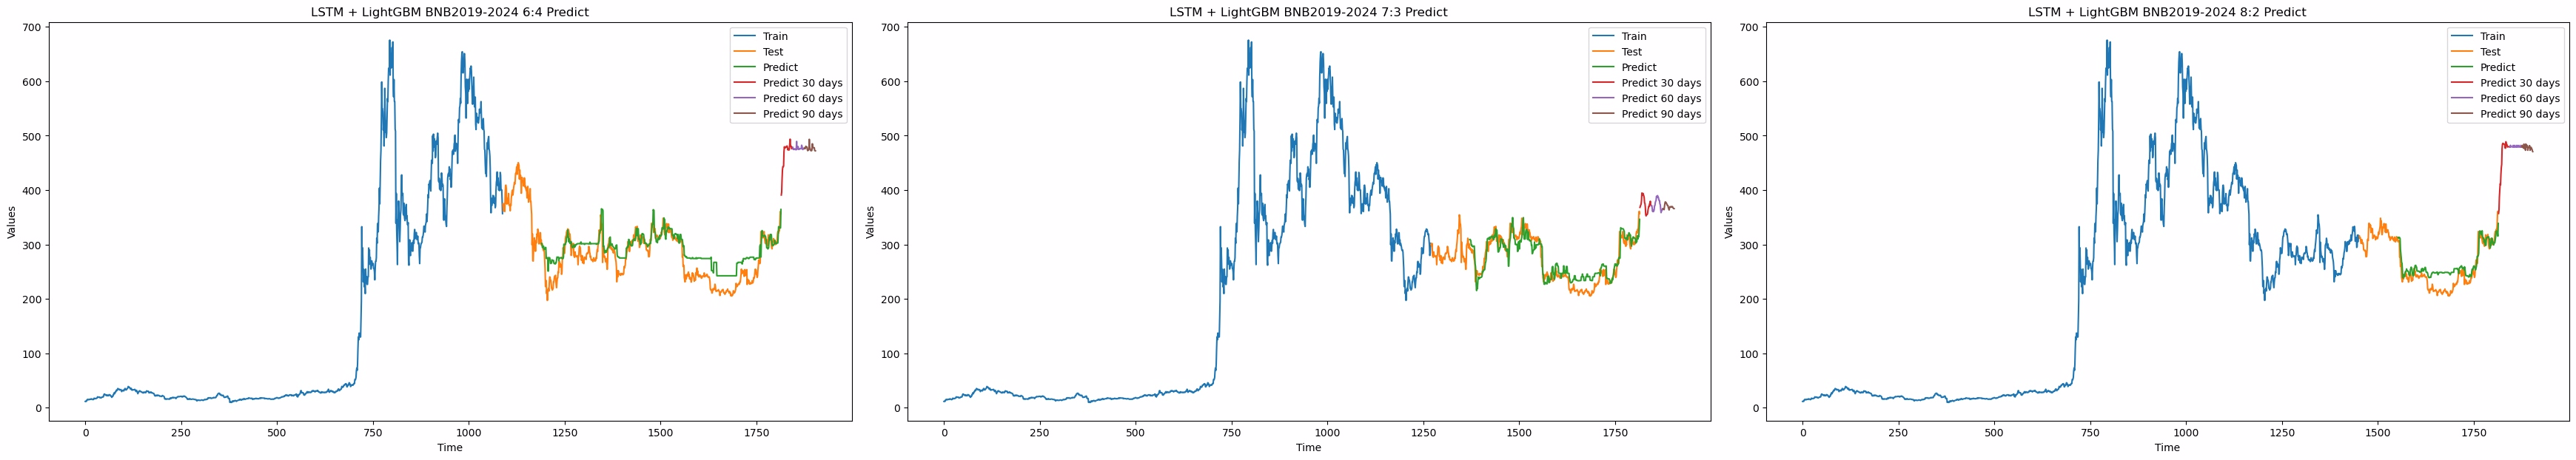
\includegraphics[width=0.5\textwidth]{bibliography/pictures/BNB LightGBM.jpg}
    \caption{Kết quả dự đoán giá Binance của LightGBM.}
\end{figure}
\begin{figure}[H]
    \centering
    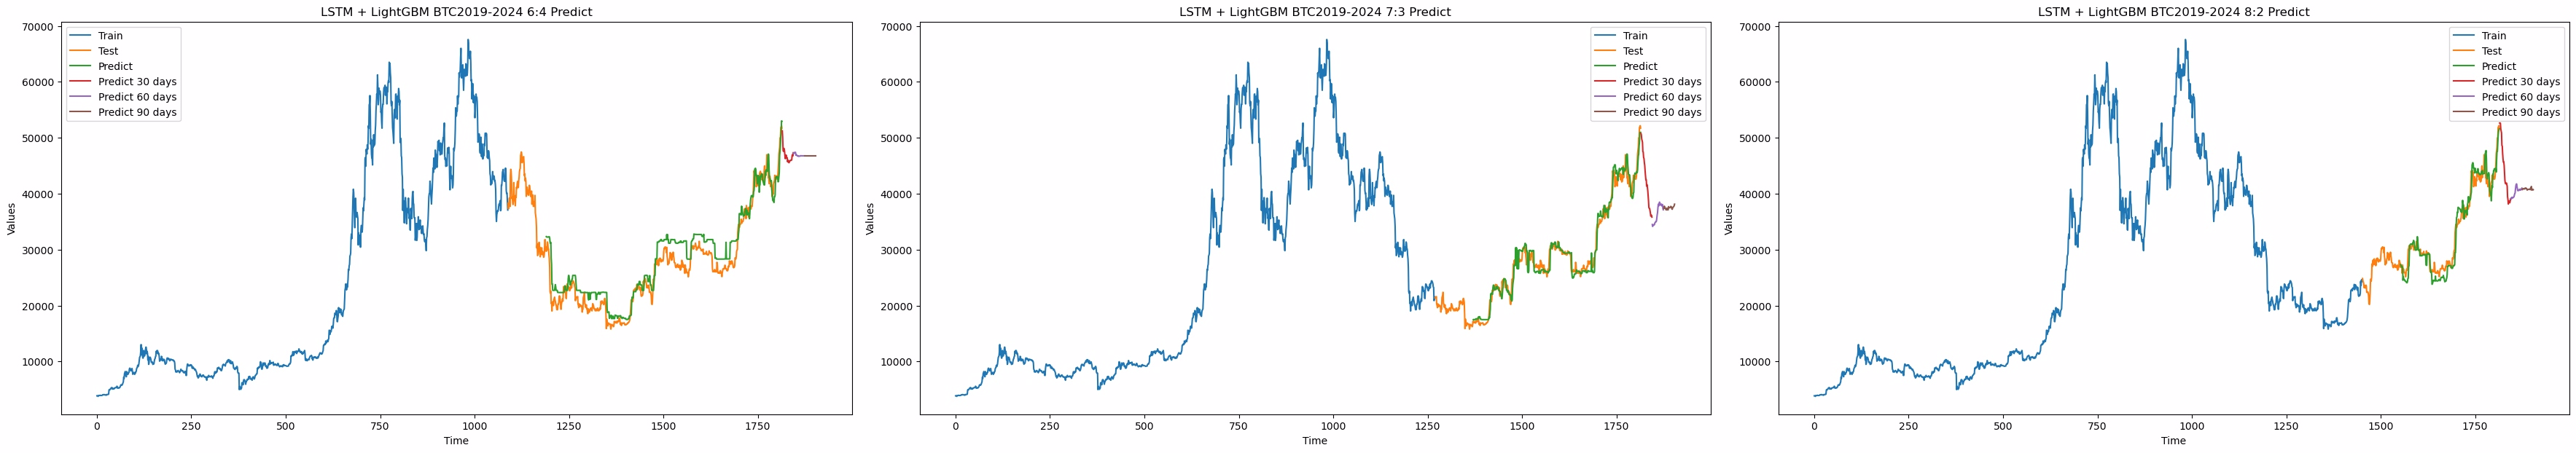
\includegraphics[width=0.5\textwidth]{bibliography/pictures/BTC LightGBM.jpg}
    \caption{Kết quả dự đoán giá Bitcoin của LightGBM.}
\end{figure}


\subsubsection{Bagging Model-Random Forest}

\begin{figure}[H]
    \centering
    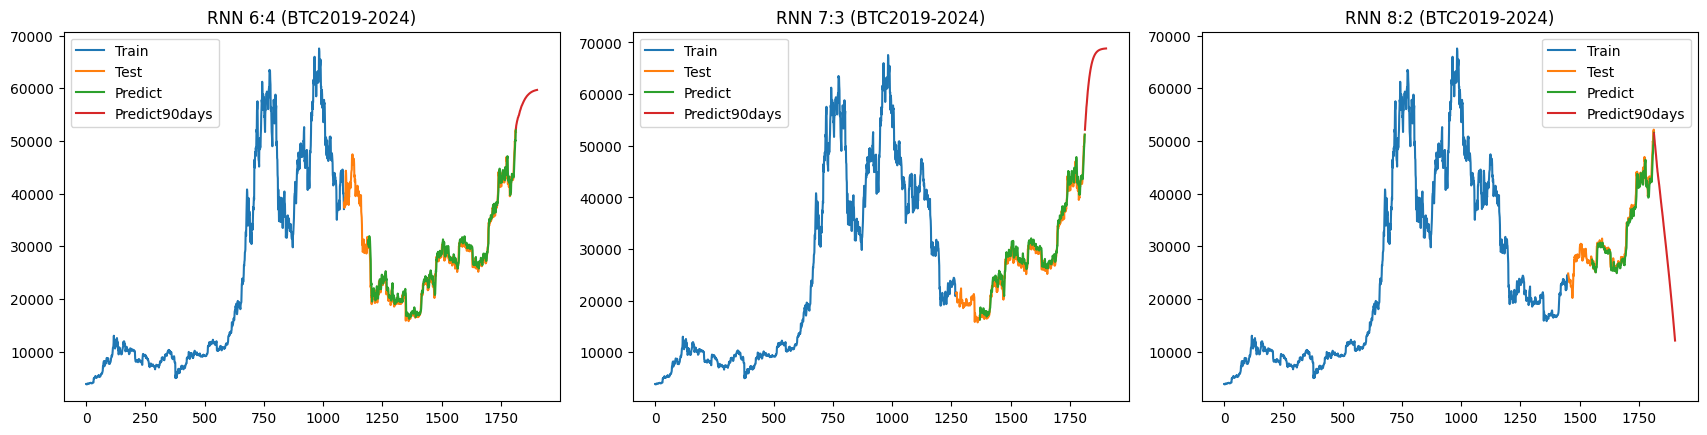
\includegraphics[width=0.5\textwidth]{bibliography/pictures/RNNbtc.png}
    \caption{Kết quả dự đoán giá Bitcoin của RNN.}
\end{figure}
\begin{figure}[H]
    \centering
    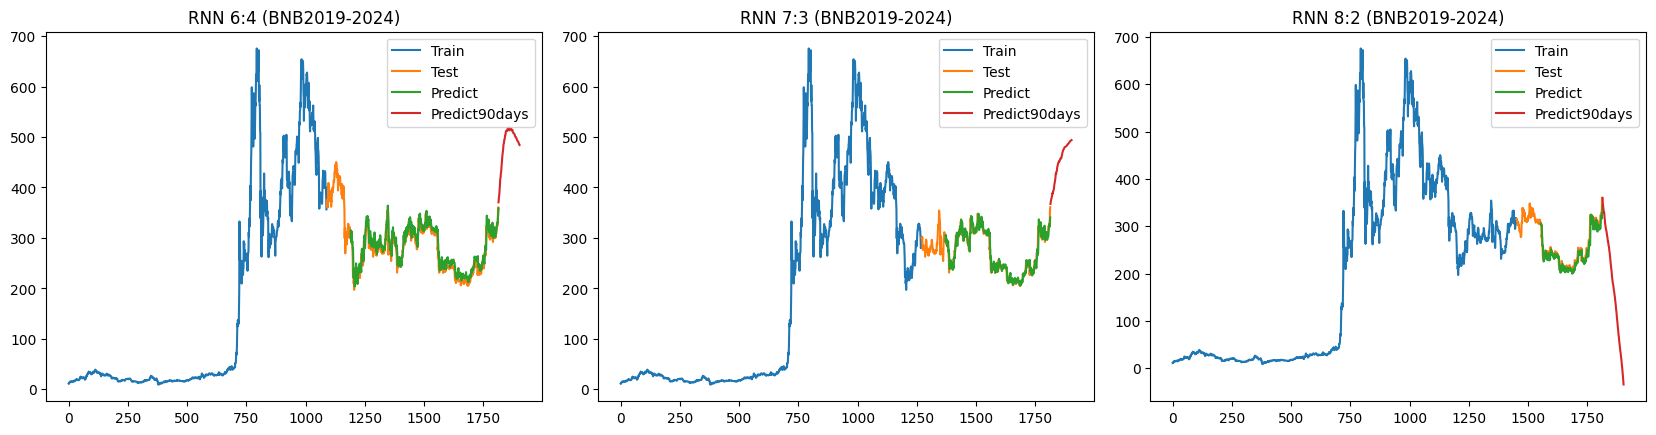
\includegraphics[width=0.5\textwidth]{bibliography/pictures/RNNbnb.png}
    \caption{Kết quả dự đoán giá Binance của RNN.}
\end{figure}
\begin{figure}[H]
    \centering
    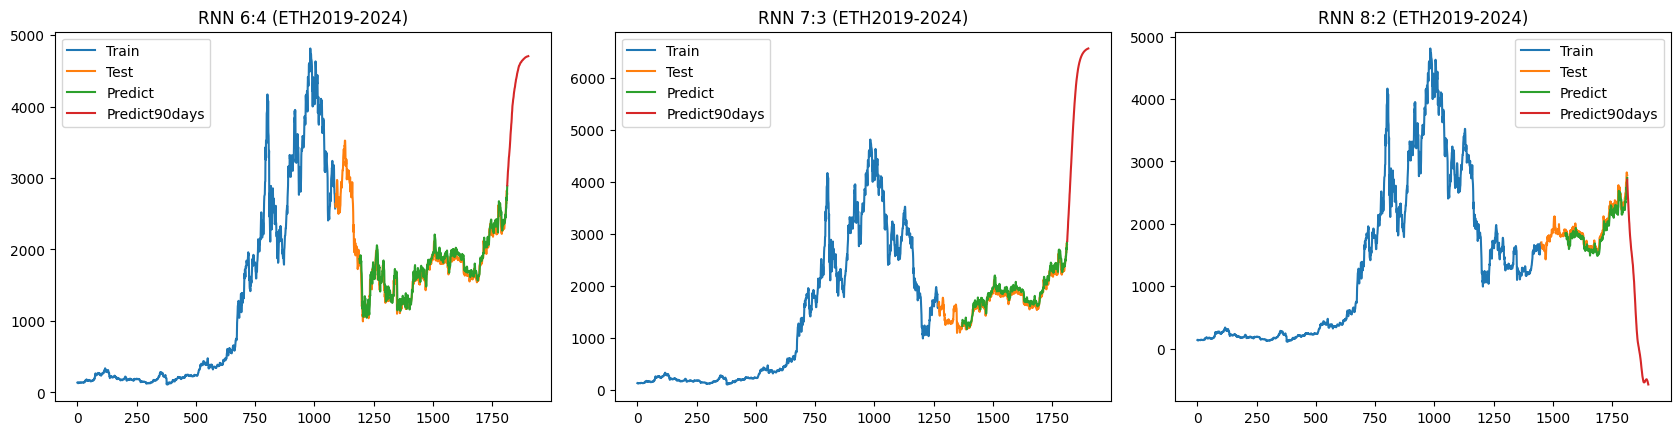
\includegraphics[width=0.5\textwidth]{bibliography/pictures/RNNeth.png}
    \caption{Kết quả dự đoán giá Ethereum của RNN.}
\end{figure}

\subsubsection{Linear Regression}
\begin{figure}[H]
    \centering
    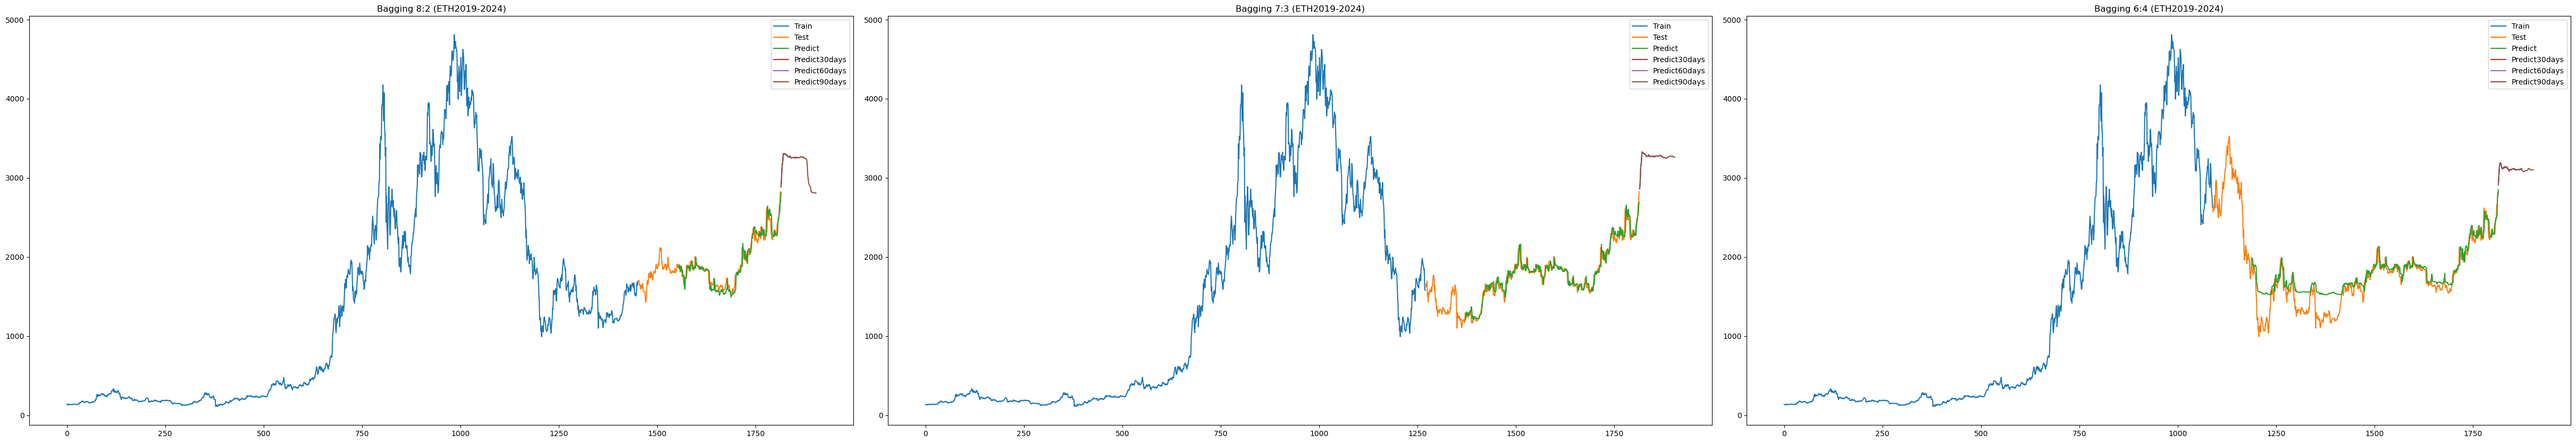
\includegraphics[width=0.5\textwidth]{bibliography/pictures/Bagging_ETH.png}
    \caption{Kết quả dự đoán giá Ethereum của Bagging Model.}
\end{figure}
\begin{figure}[H]
    \centering
    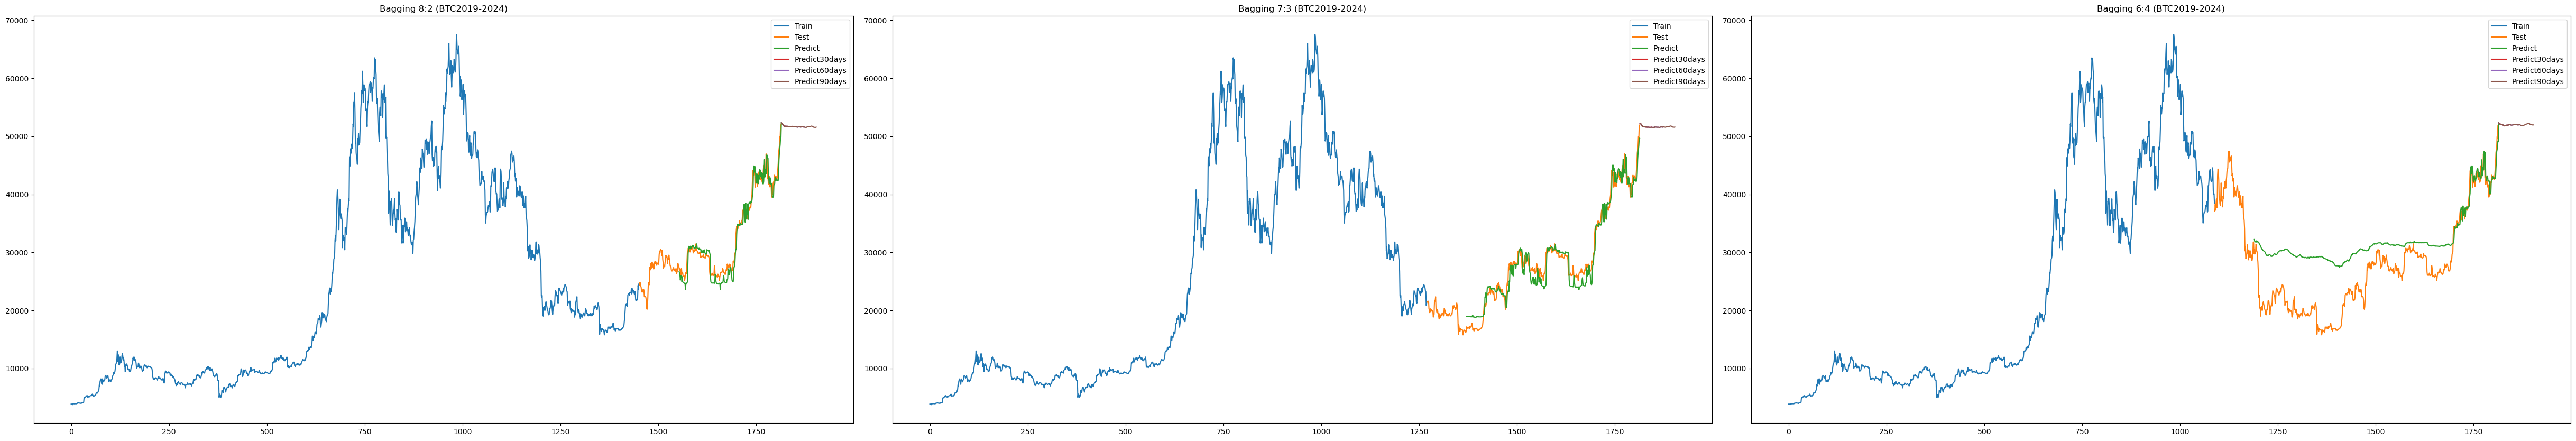
\includegraphics[width=0.5\textwidth]{bibliography/pictures/Bagging_BTC.png}
    \caption{Kết quả dự đoán giá Bitcoin của Bagging Model.}
\end{figure}
\begin{figure}[H]
    \centering
    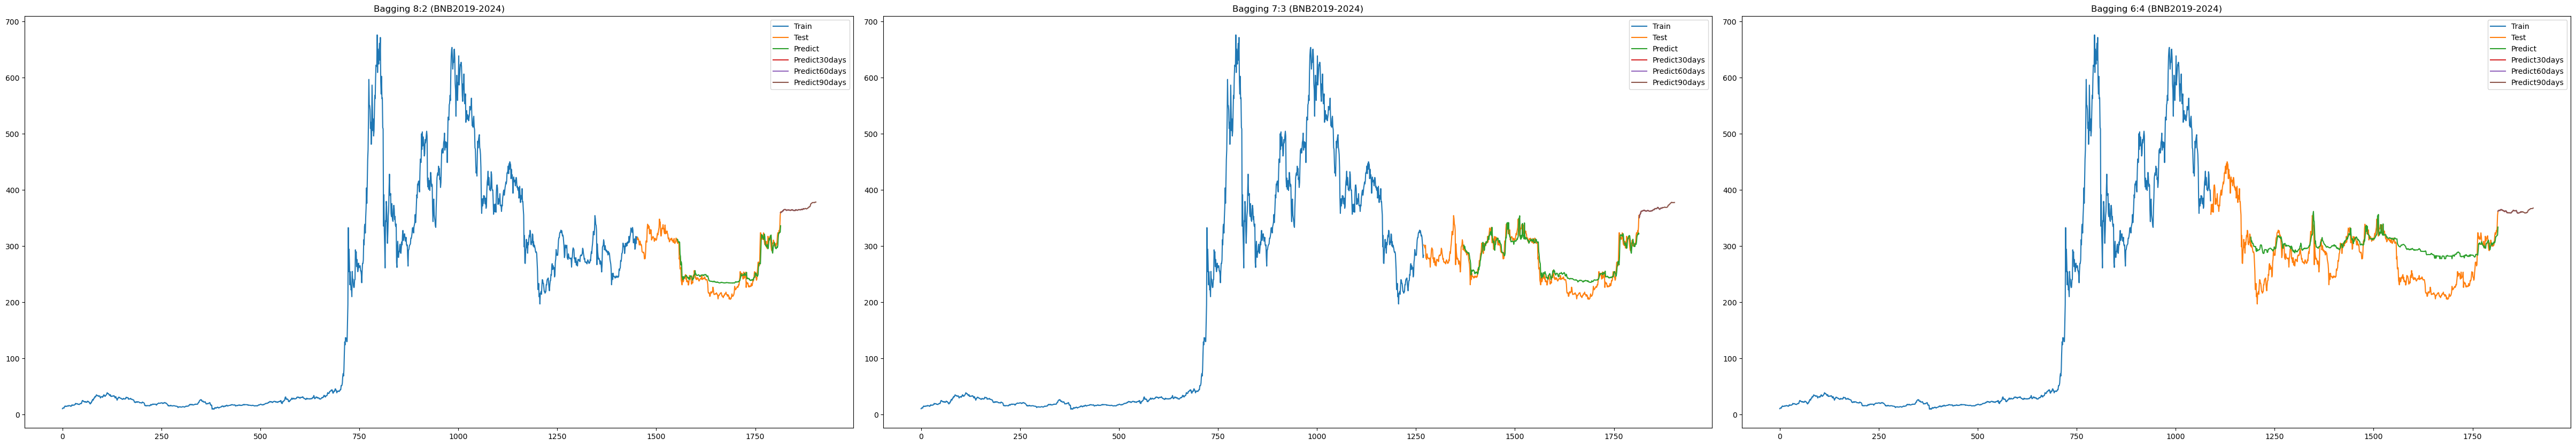
\includegraphics[width=0.5\textwidth]{bibliography/pictures/Bagging_BNB.png}
    \caption{Kết quả dự đoán giá Binance của Bagging Model.}
\end{figure}

\subsubsection{PatchTST}

\begin{figure}[H]
    \centering
    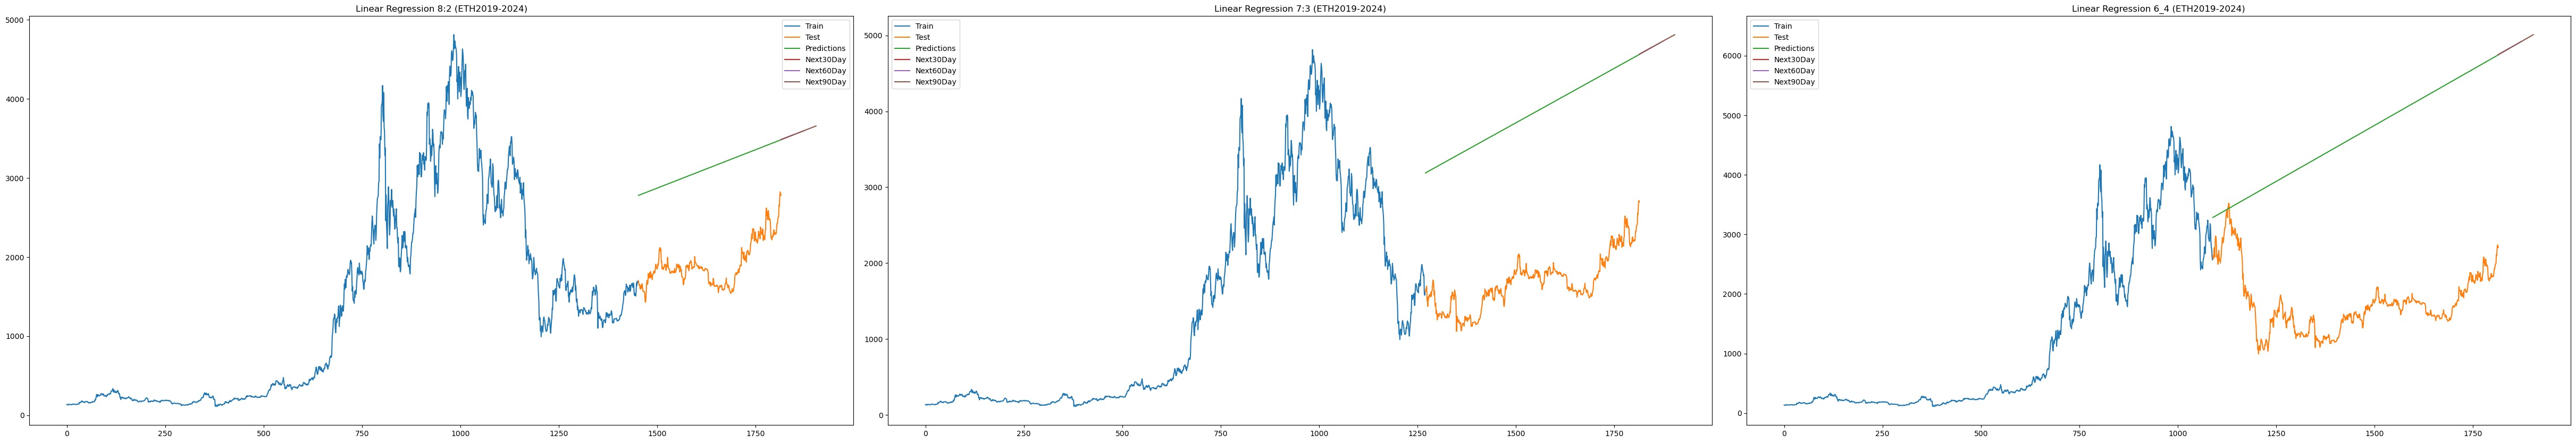
\includegraphics[width=0.5\textwidth]{bibliography/pictures/LinearRegression_ETH.png}
    \caption{Kết quả dự đoán giá Ethereum của Linear Regression.}
\end{figure}
\begin{figure}[H]
    \centering
    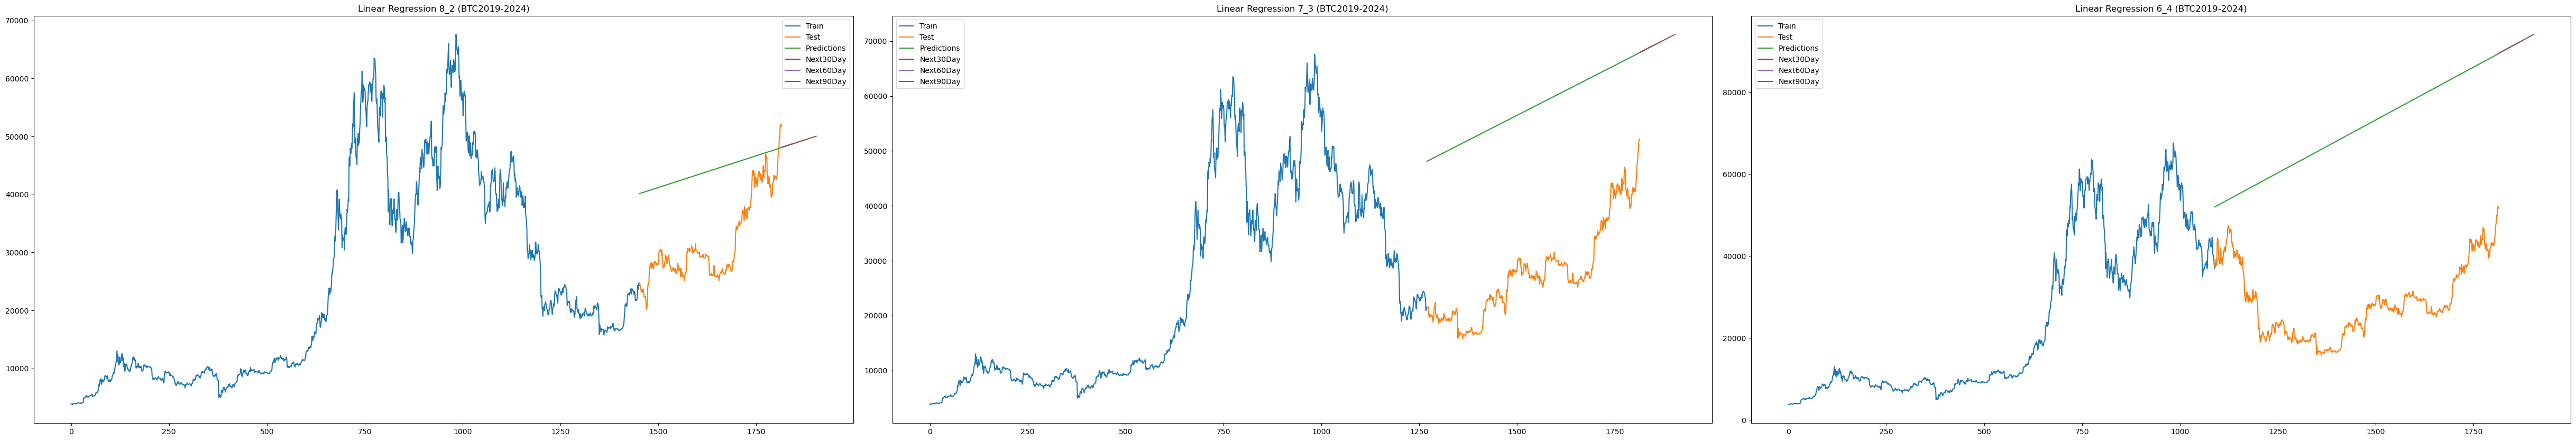
\includegraphics[width=0.5\textwidth]{bibliography/pictures/LinearRegression_BTC.png}
    \caption{Kết quả dự đoán giá Bitcoin của Linear Regression.}
\end{figure}
\begin{figure}[H]
    \centering
    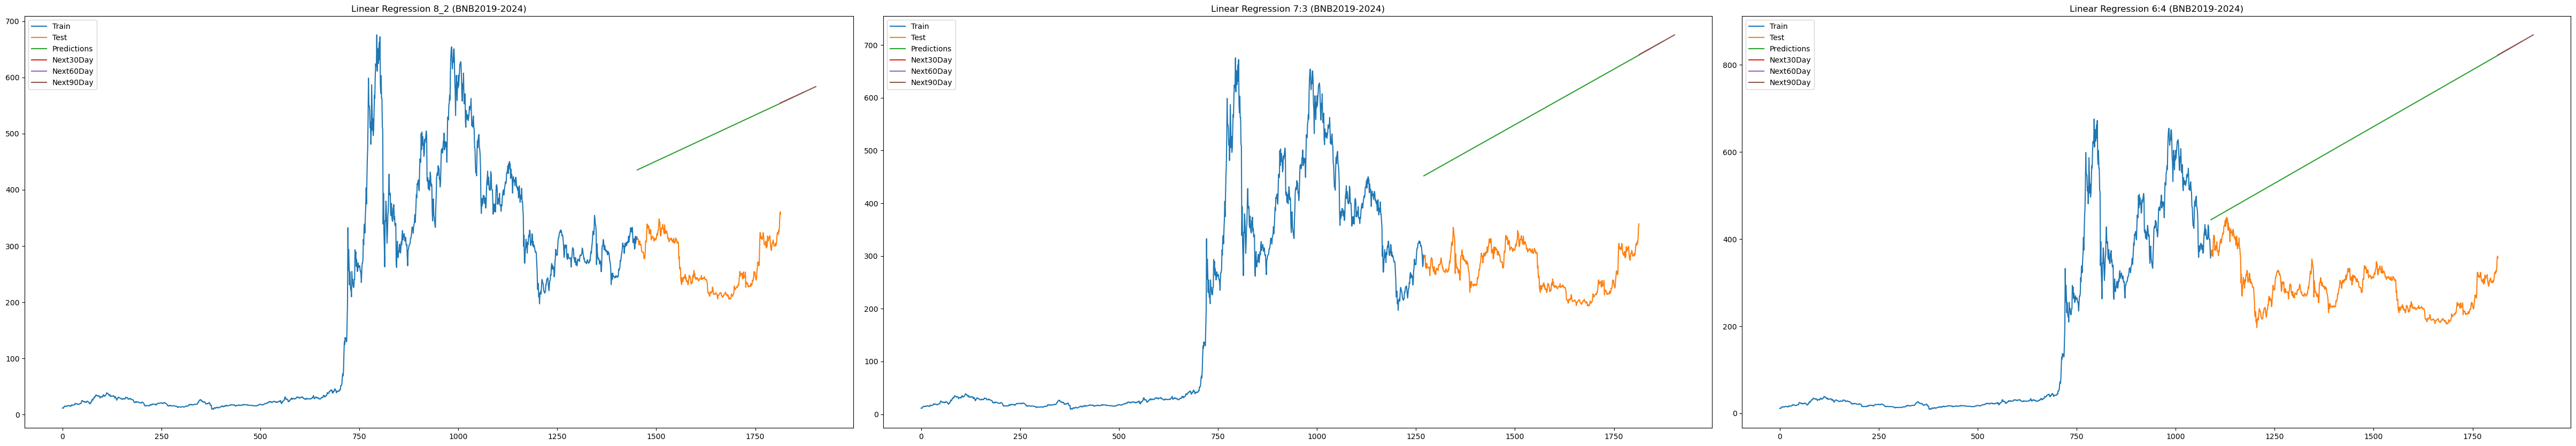
\includegraphics[width=0.5\textwidth]{bibliography/pictures/LinearRegression_BNB.png}
    \caption{Kết quả dự đoán giá Binance của Linear Regression.}
\end{figure}



\subsubsection{Holt-Winters}

\begin{figure}[H]
    \centering
    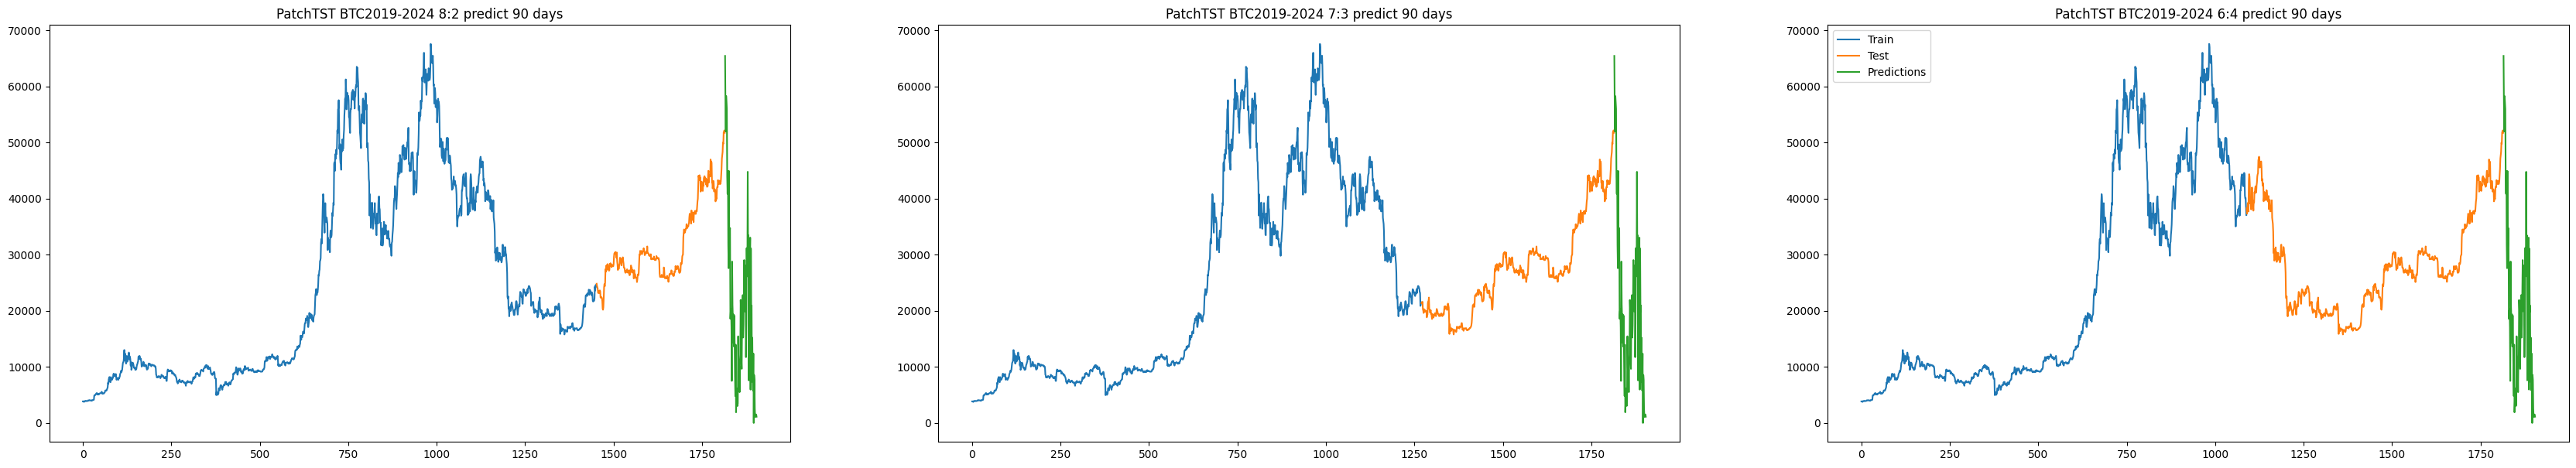
\includegraphics[width=0.5\textwidth]{bibliography/Figure/PatchTST_BTC_90.png}
    \caption{Kết quả dự đoán giá Bitcoin của PatchTST.}
\end{figure}
\begin{figure}[H]
    \centering
    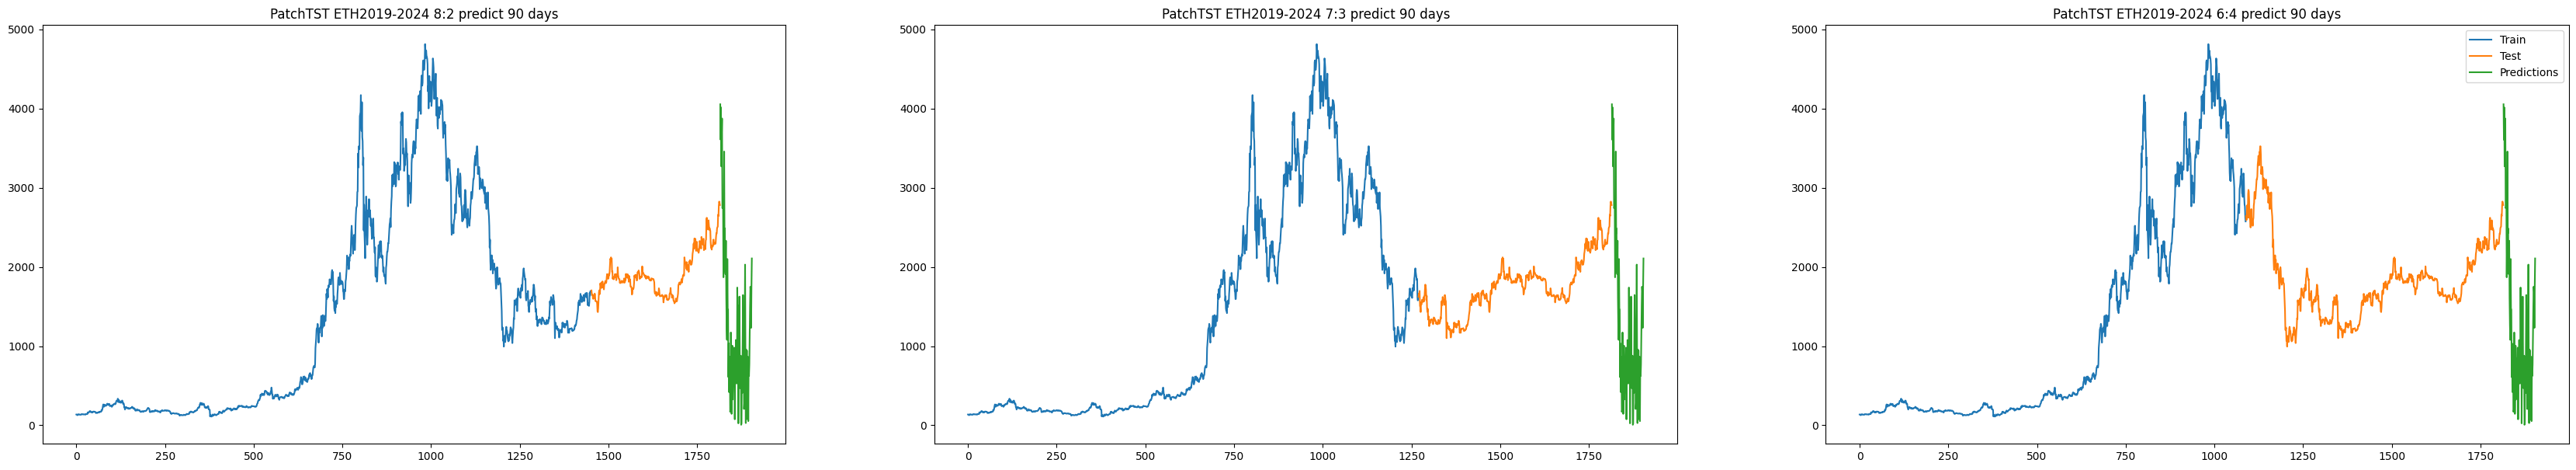
\includegraphics[width=0.5\textwidth]{bibliography/Figure/PatchTST_ETH_90.png}
    \caption{Kết quả dự đoán giá Ethereum của PatchTST.}
\end{figure}
\begin{figure}[H]
    \centering
    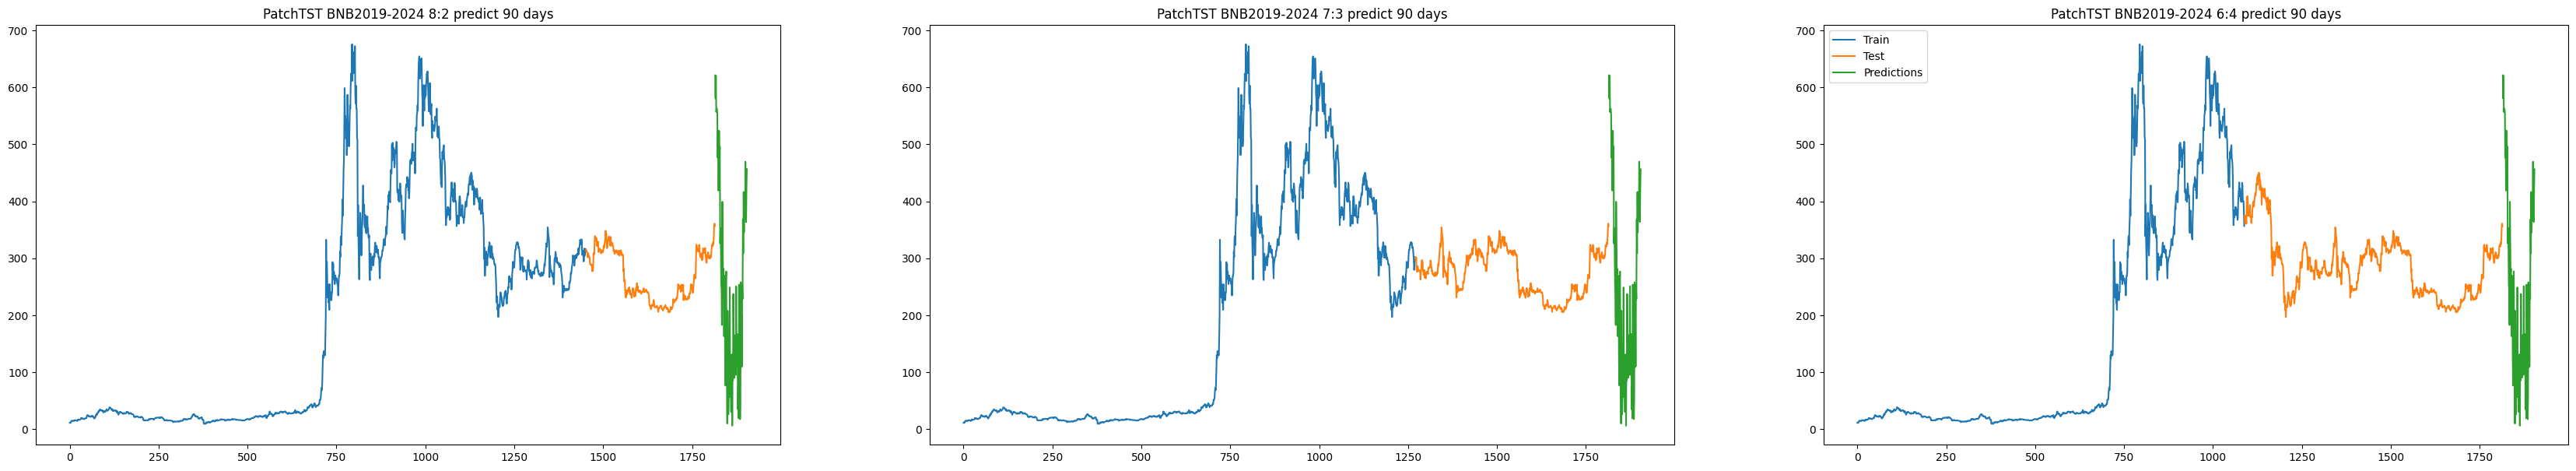
\includegraphics[width=0.5\textwidth]{bibliography/Figure/PatchTST_BNB_90.png}
    \caption{Kết quả dự đoán giá Binance của PatchTST.}
\end{figure}




\subsubsection{}
\begin{figure}[H]
    \centering
    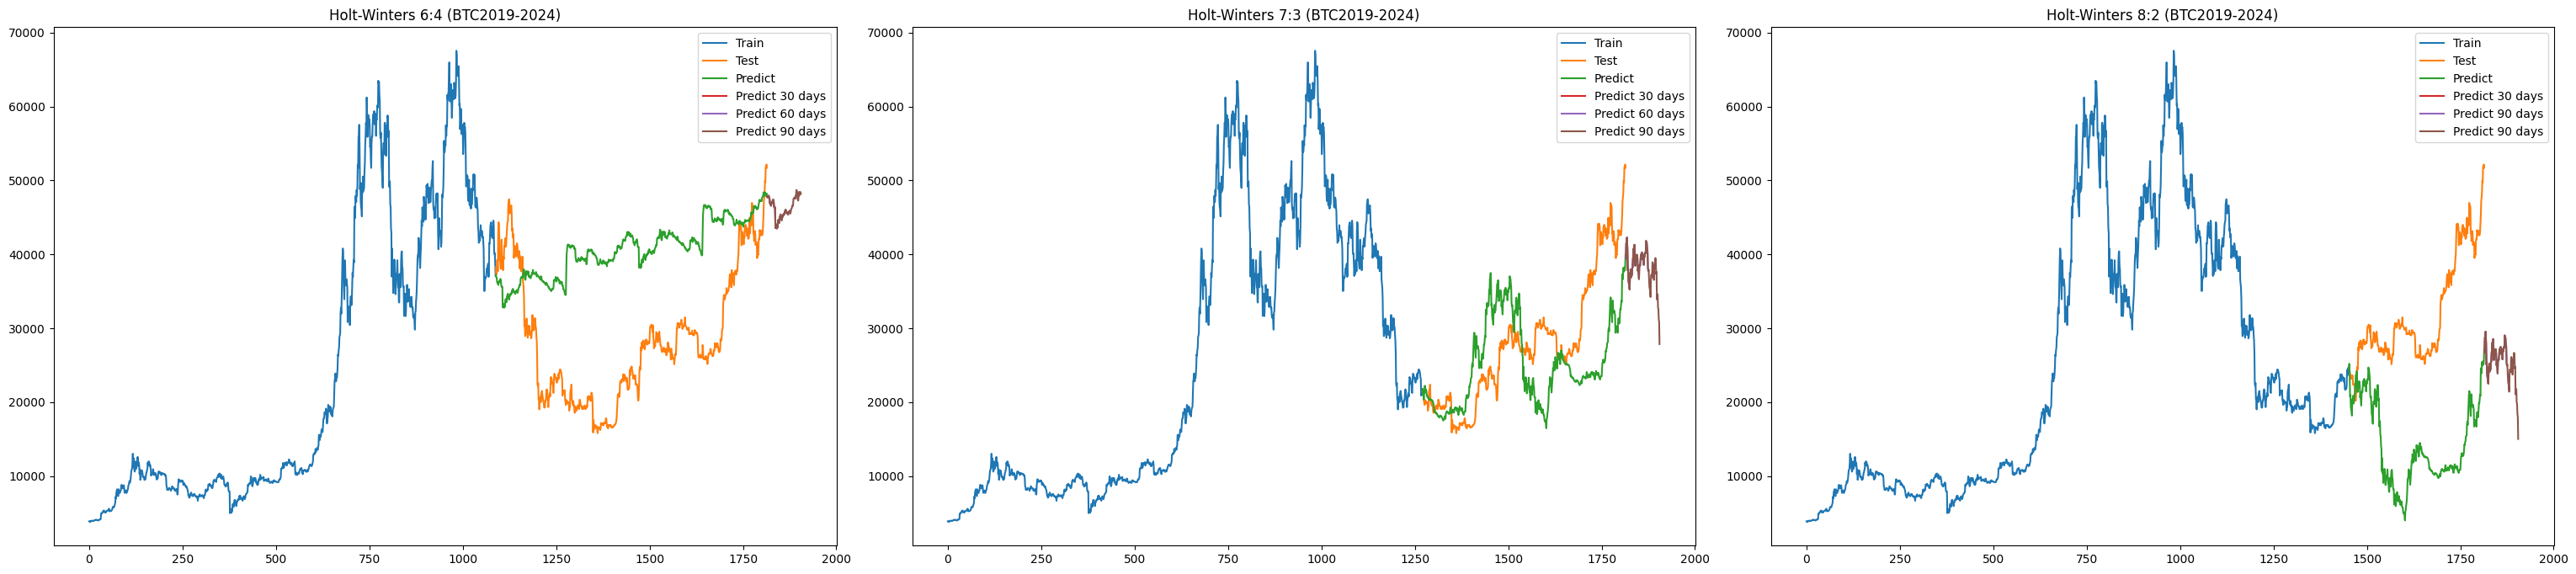
\includegraphics[width=0.5\textwidth]{bibliography/pictures/HWbtc.png}
    \caption{Kết quả dự đoán giá Bitcoin của Holt-Winters.}
\end{figure}
\begin{figure}[H]
    \centering
    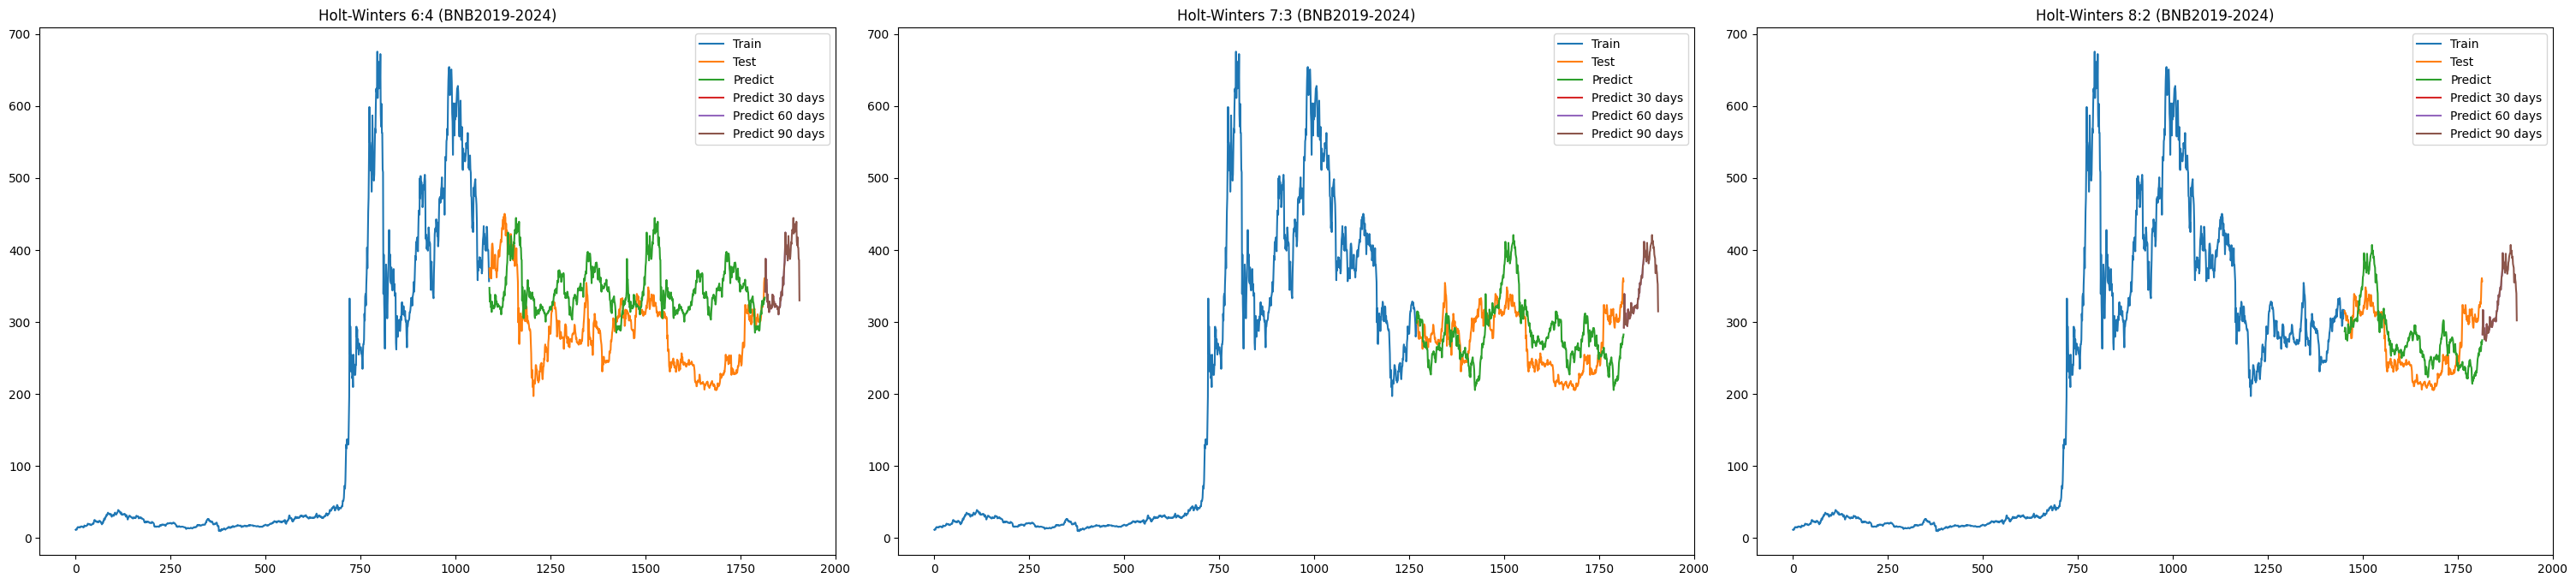
\includegraphics[width=0.5\textwidth]{bibliography/pictures/HWbnb.png}
    \caption{Kết quả dự đoán giá Binance của Holt-Winters.}
\end{figure}
\begin{figure}[H]
    \centering
    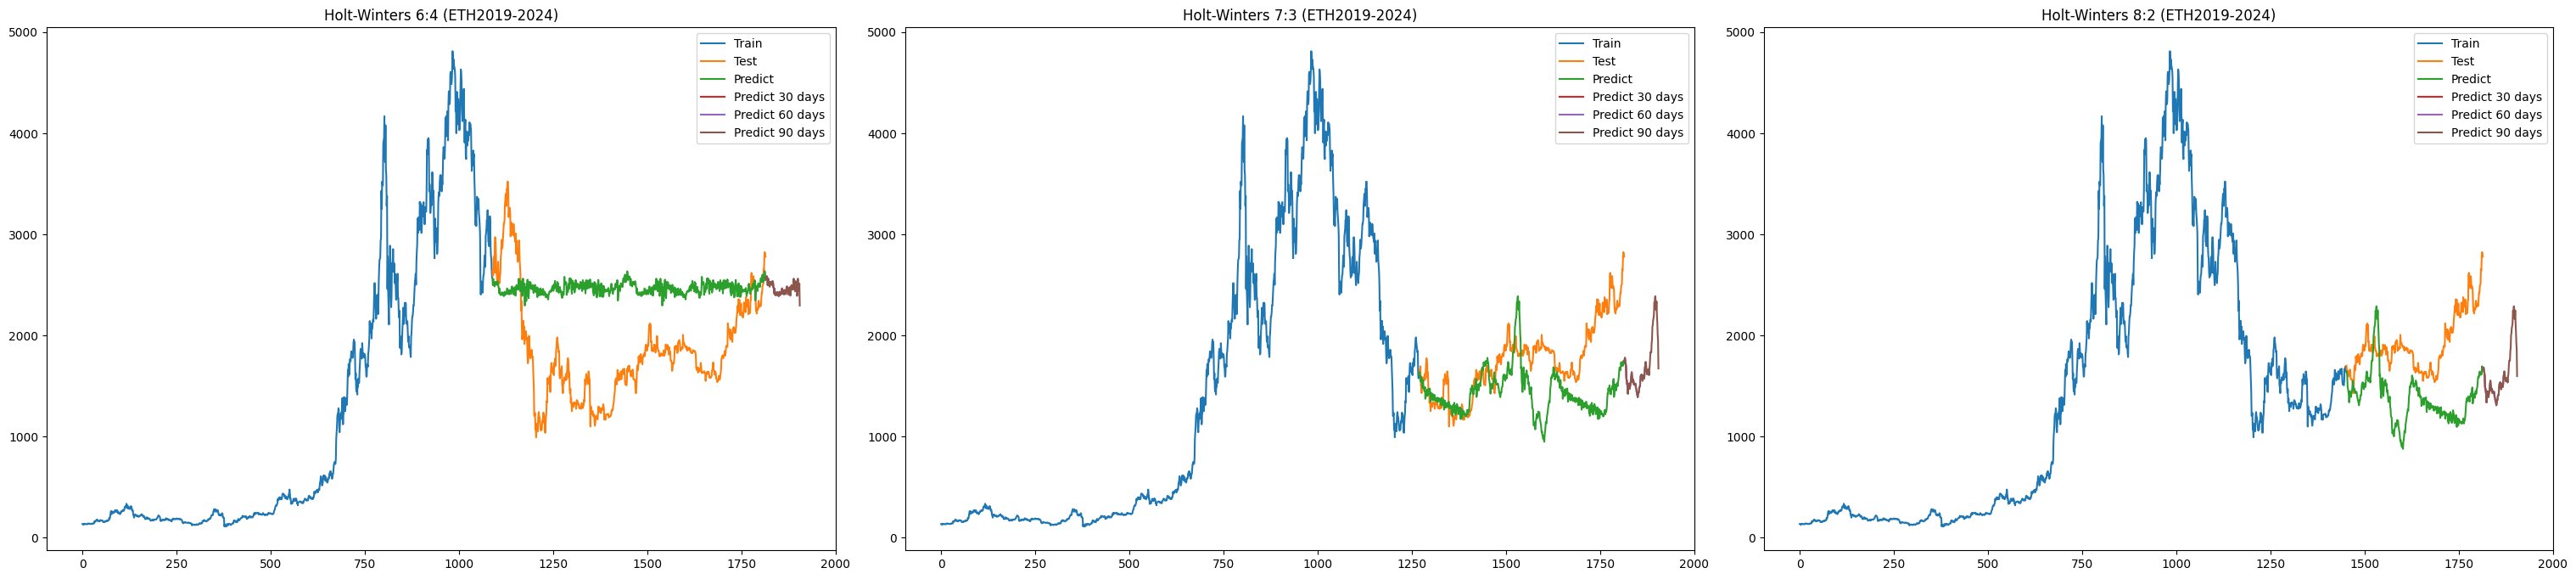
\includegraphics[width=0.5\textwidth]{bibliography/pictures/HWeth.png}
    \caption{Kết quả dự đoán giá Ethereum của Holt-Winters.}
\end{figure}

\subsection{Result} 
\begin{table}[H]
\centering
\small
\setlength{\tabcolsep}{0.5pt} 
\begin{tabular}{|l|c||c||c||c||c||c||c||c||c||c|}
\hline
& & \multicolumn{3}{c|}{\textbf{BTC}} & \multicolumn{3}{c|}{\textbf{BNB}} & \multicolumn{3}{c|}{\textbf{ETH}} \\
\hline
\textbf{Model} & \textbf{Ratio} & \textbf{RMSE} & \textbf{MSE} & \textbf{MAPE} & \textbf{RMSE} & \textbf{MSE} & \textbf{MAPE} & \textbf{RMSE} & \textbf{MSE} & \textbf{MAPE} \\
\hline
LR   & 8:2 & 13281.713 & 176403905.368 & 43.153 & 234.894 & 55175.340 & 89.849 & 1234.472 &  1523921.362 & 65.752\\
    & 7:3 & 30575.467 & 934859201.08 & 122.062 & 304.966 & 93004.572 & 112.332 & 2241.142  & 5022717.602 & 132.291 \\
    & 6:4 & 43631.231 & 1903684403.160 & 165.277 & 2958.333 & 8751735.592 & 167.497 & 374.496 & 140247.836 & 131.028  \\
\hline
Holt-Winters & 8:2 & 19494.104 & 380020103.158 & 53.556 & 45.172 & 2040.467 & 14.586 & 654.421 & 428266.346 & 27.918 \\
    & 7:3 & 8332.365 & 69428298.686 & 22.415 & 48.647 & 2366.593 & 15.284 & 486.518 & 236699.316 & 18.258  \\
    & 6:4 & 14734.705 & 217111528.885 & 56.744 & 80.598 & 6496.047 & 26.587 & 803.522 & 645648.138 & 46.334 \\
\hline
RNN & 8:2 & 34092.126 & 1162273044.790 & 7467700.375 & 247.497 & 61255.012 & 69187.291 & 1913.928 & 3663119.549 & 493447.914 \\
    & 7:3 & 31362.461 & 983603991.239 & 8265002.602 & 275.301 & 75790.684 & 71076.489 & 1911.257 & 3652903.898 & 537458.234 \\
    & 6:4 & 28665.271 & 821697745.549 & 8379727.686 & 283.409 & 80320.761 & 72649.295 & 1793.959 & 3218289.393 & 543341.059 \\
\hline
ARIMA & 8:2 & 0.325 & 0.106 & 0.025 & 0.233 & 0.054 & 0.034 & 0.184 & 0.034 & 0.018 \\
    & 7:3 & 0.360 & 0.129 & 0.028 & 0.184 & 0.034 & 0.026 & 0.204 & 0.042 & 0.022 \\
    & 6:4 & 0.423 & 0.179 & 0.036 & 0.239 & 0.057 & 0.036 & 0.448 & 0.201 & 0.054 \\
\hline
LightGBM & 8:2 & 1473.369 & 2170816.998 & 0.036 & 20.534 & 421.661 & 0.072 & 73.275 & 5369.22 & 0.028  \\
    & 7:3 & 1127.487 & 1271225.997 & 0.030 & 15.441 & 238.423 & 0.05 & 82.763 & 6849.698 & 0.039  \\
    & 6:4 & 2388.382 & 5704367.035 & 0.080 & 25.827 & 667.052 & 0.085 & 171.231 & 29320.010 & 0.094  \\
\hline
GRU & 8:2 &1871.52  &3391223  &0.038 &12.9796 &168.47 &0.0309 &94.8131 &8989.53 &0.0343 \\
    & 7:3 &1550.66  &2404555  &0.043 &14.9132 &222.40 &0.0384 &96.6455 &9340.36 &0.040 \\
    & 6:4 &10072.2  &101447619  &0.3925 &21.0943 &966.85 &0.1026 &150.521 &22656.89 &0.069 \\
\hline
Gradient Boosting & 8:2 &4.6388  &21.5186  &0.0078 &4.1578 &17.2879 &71666 &4.3371 &18.8108 &63776 \\
    & 7:3 &4.7361  &22.4314  &0.0079 &4.6055 &21.2106 &48754 &4.5189 &20.4210 &25883 \\
     & 6:4 &4.6958  &22.0514  &0.0084 &4.5139 &20.375 &40860 &4.8312 &22.3450 &48824 \\
\hline
BG & 8:2 & 0.044 & 0.002 & 9.015 & 0.0202 & 0.0004 & 4.817 &  0.0131 & 0.0002& 2.533\\
    & 7:3 &  0.022 & 0.0005 & 5.378 &  0.02009 & 0.0004 & 4.351 & 0.0109 & 0.0001 & 2.143 \\
    & 6:4 & 0.102 & 0.0106 & 31.109 & 0.058 & 0.0034 & 13.131 & 0.102 & 0.0106 & 31.109 \\
\hline
LSTM & 8:2 & 35206.264 & 1239481042.236 & 7710365.511 & 247.261 & 61138.072 & 69184.116 & 1918.097 & 3679095.877 & 494731.584    \\
    & 7:3 & 31390.871 & 985386792.539 & 8261187.272 & 267.204 & 71397.962 & 69034.377 & 1828.836 & 3344642.186 & 514292.382   \\
    & 6:4 & 28619.752 & 819090215.224 & 8372540.489 & 270.585 & 73216.161 & 69372.351 & 1754.844 & 3079477.977 & 532363.836   \\
\hline
PatchTST & 8:2 & 28742.968 & 24872.653 & 1.798 & 226.754 & 201.147 & 0.512 & 1680.91 & 1279.968 & 2.045 \\
    & 7:3 & 30777.957 & 27351.518 & 2.075 & 252.552 & 221.203 & 0.652 & 1719.241 & 1528.288 & 2.325 \\
    & 6:4 & 33879.124 & 31856.856 & 2.987 & 289.531 & 267.517 & 0.756 & 2078.865 & 1618.786 & 2.856 \\
\hline
\end{tabular}
\caption{Kết quả chỉ số đánh giá RMSE, MAPE và MSE trên ba Dataset}
\end{table}    

\section{Conclusion}
Từ kết quả so sánh của Bảng II, dựa vào độ đo RMSE, MAPE và MSE có thể thấy mô hình GRU và Bagging Model có kết quả tốt nhất trong các mô hình ở 3 dataset. Kết quả nghiên cứu này cho thấy thuật toán GRU và Bagging Model là phù hợp nhất trong việc dự đoán giá tiền ảo trong tương lai của 3 loại tiền ảo Bitcoin, Binance và Ethereum. Nghiên cứu này nhấn mạnh sự cần thiết của việc sử dụng nhiều phương pháp mô hình hóa trong phân tích tài chính, ngoài ra mô hình ARIMA có tiềm năng trong việc dự báo giá tiền ảo. Do đó, nhóm cũng sẽ xem xét trên 3 độ đo và kết luận hai mô hình cho kết quả tốt nhất là GRU và Bagging Model nhằm báo giá 30 ngày tiếp theo của cả ba tiền ảo.
\section*{Acknowledgment}
Với lòng biết ơn sâu sắc nhất, nhóm xin gửi lời cảm ơn chân thành đến quý Thầy Cô và các giảng viên đã giúp đỡ chúng em trong quá trình thực hiện đề tài này. Nhóm cũng xin gửi lời cảm ơn đến thầy Nguyễn Đình Thuân – giảng viên lý thuyết môn Phân tích dữ liệu kinh doanh và anh Nguyễn Minh Nhựt – trợ giảng của môn đã tận tình hướng dẫn và hỗ trợ nhóm trong suốt quá trình làm đồ án. Nhờ sự hướng dẫn của các thầy và anh, nhóm đã tiếp thu được nhiều kiến thức bổ ích và hoàn thành đồ án một cách tốt nhất.
\clearpage
\begin{thebibliography}{00}
\bibitem{b1} Nakamoto, S. Bitcoin: A Peer-to-Peer Electronic Cash System. Technical Report. Available online: https://bitcoin.org/bitcoin.pdf.
\bibitem{b2} F. Reid and M. Harrigan, “An Analysis of Anonymity in the Bitcoin System,” Tech. Rep., 2011.[Online]. Available: http://arxiv.org/abs/1107.4524.
\bibitem{b3} P. N. Sureshbhai, P. Bhattacharya, and S. Tanwar, "aRuNa: A blockchainbased sentiment analysis framework for fraud cryptocurrency schemes," in Proc. IEEE Int. Conf. Commun. 
\bibitem{b4} Suhwan Ji, Jongmin Kim and Hyeonseung Im, "A Comparative Study of Bitcoin Price Prediction Using Deep Learning" in Mathematics 2019, 7, 898; doi:10.3390/math7100898.
\bibitem{b5} SUDEEP TANWAR 1, (Senior Member, IEEE), NISARG P. PATEL 1
,SMIT N. PATEL 2, JIL R. PATEL 3, GULSHAN SHARMA 4, AND INNOCENT E. DAVIDSON 4, (Senior Member, IEEE), "Deep Learning-Based Cryptocurrency
Price Prediction Scheme With Inter-Dependent Relations" in Digital Object Identifier 10.1109/ACCESS.2021.3117848.
\bibitem{b6} Financial Platform and News Website. Accessed: 2008. [Online]. Available: https://www.investing.com/.
\bibitem{b7} V. Derbentsev, N. Datsenko, O. Stepanenko, and V. Bezkorovainyi,'Forecasting cryptocurrency prices time series using machine learning approach," SHS Web Conf., vol. 65, Jan. 2019, Art. no. 02001.
\bibitem{b8} Iqbal H. Sarker, Machine Learning: Algorithms, Real‑World Applications and Research. Available: https://link.springer.com/article/10.1007/s42979-021-00592-x
Directions
\bibitem{b9} Cristescu, R. and Popescu, M. (2019). Short-term cryptocurrency price prediction using gradient boosting machines. IEEE Xplore, 1-4. Available: https://ieeexplore.ieee.org/document/9964870

\bibitem{b10} Huang, S., Wang, W., Dong, Z. and Wang, Y. (2020). LightGBM and LSTM Based Cryptocurrency Price Prediction. Available: https://arxiv.org/abs/2403.03410.

\bibitem{b11} Shen, Z., Wang, Y., and Liu, R. (2018). Short-term and long-term cryptocurrency price prediction using Holt-Winters exponential smoothing. IEEE Transactions on Computational Intelligence and AI in Robotics and Automation, 4(1), 74-81. Available: https://ieeexplore.ieee.org/document/9257664.
\bibitem{b12} Li, Y., Zhang, W., and Liu, P. (2023). PatchTST: A Transformer-based Spatio-Temporal Shifted Transformer for Short-Term Bitcoin Price Forecasting. Available: https://arxiv.org/abs/2303.04983

\end{thebibliography}
\vspace{12pt}
\end{document}
